\documentclass[a4]{llncs}

% \usepackage{latexsym}
%\usepackage{amsmath}
\usepackage{xspace}
\usepackage{url}
%\usepackage{alltt}
%\usepackage{amssymb}
%\usepackage{epsfig}
\usepackage{listings}
%\usepackage{longtable}

\usepackage[T1]{fontenc}
\usepackage[latin1]{inputenc}


\def \bsl       {\symbol{92}}
\def \unsc      {\symbol{95}}

\def\lstlanguagefiles{../../THESIS/Jml.sty}
\lstloadlanguages{Jml}
\lstset{language=Jml,flexiblecolumns=false}


\newcommand{\LST}{\ensuremath{\mathsf{G}}}
\newcommand{\MST}{\ensuremath{\mathsf{M}}}
\newcommand{\Anno}{\ensuremath{\mathsf{Q}}}

\newcommand{\JudgeF}[4]{\ensuremath{\LST,\Anno \vdash \lbrace {#2} \rbrace\, {#1}\, \lbrace {#3} \rbrace\, ({#4})}}

\newcommand{\ppt}{\ensuremath{\mathit{pc}}}


\newcommand{\sem}[1]{\ensuremath{[\![{#1}]\!]_{\small{\textit{BML}}}\/}}

\newcommand{\mobius}{\textsf{MOBIUS}\xspace}

\newcommand{\varHook}[1]{\mbox{\slshape #1}}
\newcommand{\codeHook}[1]{\mbox{\ttfamily #1}}



%%%%%%%%%%%%%%%%%%%%%%%%%%%%%%%%%%%%%%%%%%%%%%%%%%%%%%%%%%%%%%%%%%%%%%%%%%%%%%%%%%%%%%%%%%%%%%%%%%%%%%
%%%%%%%%%%%%%%%%%%%%%%%%%%%%%%%%%%%%%%%%BYTECODE LANGUAGE%%%%%%%%%%%%%%%%%%%%%%%%%%%%%%%%%%%%%%%%%%%%%%%%%%%
%%%%%%%%%%%%%%%%%%%%%%%%%%%%%%%%%%%%%%%%%%%%%%%%%%%%%%%%%%%%%%%%%%%%%%%%%%%%%%%%%%%%%%%%%%%%%%%%%%%%%%%%%%%%
% \newcommand{\bcIns}{\mbox{ \rm I} }
% \newcommand{\instrs}{\mbox{ \rm IS} }
% \newcommand{\ifCond}{ \instr{if\_cond } }
% \newcommand{\goto}{ \instr{goto } }
% \newcommand{\return}{ \instr{return } }
% \newcommand{\arithOp}{ \instr{arith\_op} }
% \newcommand{\load}{ \instr{load} }
% \newcommand{\store}{ \instr{store} }
% \newcommand{\push}{ \instr{push} }
% \newcommand{\pop}{\instr{pop}}
% \newcommand{\dup}{\instr{dup}}
% \newcommand{\iinc}{\instr{iinc}}
% \newcommand{\new}{\instr{new}}
% \newcommand{\newarray}{\instr{newarray}}
% \newcommand{\putfield}{\instr{putfield}} 
% \newcommand{\getfield}{\instr{getfield}}
% \newcommand{\arrstore}{\instr{type\_astore}} 
% \newcommand{\arrload}{\instr{type\_aload}}
% \newcommand{\arraylength}{\instr{arraylength}}
% \newcommand{\instanceof}{\instr{instanceof}} 
% \newcommand{\checkcast}{\instr{checkcast}} 
% \newcommand{\athrow}{\instr{athrow}}
% \newcommand{\invoke}{\instr{invoke}}
% \newcommand{\jsr}{\instr{jsr}}
% \newcommand{\ret}{\instr{ret}}
% \newcommand{\swap}{\instr{swap}}
%%%%%%%%%%%%%%%%%%%%%%%%%%%%%%%%%%%%%%%%%%%%%%%%%%%%%%%%%%%%%%%%%%%%%%%%%%%%%%%%%%%%%%%%%%%%%%%%%%%%%%
%%%%%%%%%%%%%%%%%%%%%%%%%%%%%%%%%%%%%%%%BYTECODE LANGUAGE%%%%%%%%%%%%%%%%%%%%%%%%%%%%%%%%%%%%%%%%%%%%%%%%%%%
%%%%%%%%%%%%%%%%%%%%%%%%%%%%%%%%%%%%%%%%%%%%%%%%%%%%%%%%%%%%%%%%%%%%%%%%%%%%%%%%%%%%%%%%%%%%%%%%%%%%%%%%%%%%



\newcommand{\todo}[1]{\marginpar{\baselineskip0ex\rule{2,5cm}{0.5pt}\\[0ex]{\textsf{#1}}}}
%\newcommand{\fig}[1]{ Fig.#1}
\newcommand{\jmlKey}[1]{\texttt{#1}}% wrapping jml keywords
%\newcommand{\java}[1]{\texttt{#1}}
%\newcommand{\stack}[1]{\mbox{\rm\textbf{st}}(#1)}% element on top stack 
%\newcommand{\stackOnly}{\mbox{\rm St}}
%\newcommand{\stackOnlyParam}[1]{\mbox{\rm St}(#1)}
%\newcommand{\newStack}{ \lbrack~\rbrack  } % empty stack
%\newcommand{\update}[3]{ #1 [ \oplus {#2} \rightarrow {#3} ] }

%\newcommand{\counter}{\mbox{\rm\textbf{cntr}} }
%\newcommand{\counterOnly}{\mbox{\rm Cntr} }
%\newcommand{\topStack}{\mbox{\rm cntr} }
%\newcommand{\true}{\mbox{\rm\textbf{true}} } % true from the assertion language
%\newcommand{\false}{\mbox{\rm\textbf{false}}} % false from the assertion language



%\newcommand{\instr}[1]{\mbox{  \rm #1} }

%\newcommand{\loopStart}[1]{\textbf{loop\_start$\tt{_#1}$}}
%\newcommand{\loopEnd}[1]{\textbf{loop\_end$\tt{_#1}$}}
%\newcommand{\invariant}[1]{\it{I}_{\tt{#1}}}
%\newcommand{\boucle}[1]{\texttt{#1}}
%\newcommand{\loopModifies}[1]{\textbf{Modifies}(\texttt{#1}) }
%\newcommand{\ins}[1]{#1 : \mbox{\rm\texttt{instr}}}


%\newcommand{\insOnly}{\texttt{instr}}

% the grammar for the bytecode specification language
%\newcommand{\ClassSpec}{\rm{ClassSpec}}
%\newcommand{\ClassInv}{ClassInv}
%\newcommand{\ClassHistoryConstr}{ClassHistoryConstr}

%\newcommand{\MethodSpec}{\rm{MethodSpec}}


%\newcommand{\specCase}{\textrm{SpecCase}}
%\newcommand{\requires}{requires}
%\newcommand{\ensures}{ensures}
%\newcommand{\exsures}{exsures}
%\newcommand{\modifies}{modifies}

%\newcommand{\jmlStmt}[1]{\textrm{#1}}
%\newcommand{\specExpression}{\mathcal{E}^{spec}}

%\newcommand{\interMethodSpec}{\rm{InterMethodSpec}}
%\newcommand{\loopSpec}{\rm{loopSpec}}
%\newcommand{\assert}{\rm{assert}}

%\newcommand{\ArithExpr}{\texttt{ArithmeticExp} }

%\newcommand{\JMLExpr }{\texttt{JmlExp} }


%\newcommand{\integer}{\texttt{int} }
%\newcommand{\register}[1]{\mbox{\rm\textbf{reg}}(#1)}

%\newcommand{\Mynull}{\jmlKey{null}}
%%\newcommand{\this}{\texttt{this}}
\newcommand{\fieldAccess}[2]{#1\texttt{.}#2}
\newcommand{\arrayAccess}[2]{\texttt{arrayAccess(} #1 \texttt{,} #2\texttt{)}}  
%\newcommand{\arrayAccessOnly}{\mbox{\rm arrAccess}}


%\newcommand{\loopInv}{loopInvariant}
%\newcommand{\loopMod}{loopModifies}

\newcommand{\result}{\jmlKey{\bsl result}}
%\newcommand{\old}[1]{\jmlKey{$\backslash$old(}#1\jmlKey{)}}
%\newcommand{\typeof}[1]{\jmlKey{$\backslash$typeof(}#1 \jmlKey{)}}
%\newcommand{\TYPE}{\jmlKey{TYPE} }
%\newcommand{\elemtype}[1]{ \jmlKey{$\backslash$elemtype(}#1\jmlKey{)} } 
%\newcommand{\excPost}{\psi^{exc}}

%\newcommand{\Myspace}{\phantom{aaa}}
%\newcommand{\predicate}{ \mathcal{P}} 
%\newcommand{\Myfalse}{ \textit{false} }
%\newcommand{\Mytrue}{ \textit{true} }



%% abstractCtrlFlow.tex
%\newcommand{\execRel}{\rightarrow} % the execution relation
%\newcommand{\blockm}[1]{ \tt{b^{#1}} }
%\newcommand{\blockSeq}[1]{ \tt{b_{seq}^{#1}} }
%\newcommand{\pathm}[2]{\blockm{#1} \execRel^{*} \blockm{#2} }
%\newcommand{\instrPost}[1]{ post(\instr{#1} )}





%from wp.tex
%\newcommand{\wpExeWithLoops}[1]{ \rm{Wp''}\rm{(#1)} }
%\newcommand{\wpExe}[1]{ \rm{Wp'}\rm{(#1)} }



%\newcommand{\getExcPost}{\mbox{\rm\textsf{getExcPostIns}}}
%\newcommand{\excPost}{\mbox{\rm\textsf{excPost}}}
%\newcommand{\javaNull}{null}
%\newcommand{\length}{\mbox{\rm arrLength}} % stands for array length


%%%%%%%%%%%%%%%%%%%%%%%%%%%%%%%%%%%%%%%%%%%%%%%%%%%%%%%%%%%%%%%%%%%%%%%%%%%%%%%%%%%%%%%%%%%%%%%%%%%%%%%%%%%%%%%%%%%%%%%%%%%%%%%%%%%%%%%%%%%%%%%%%%%%%%%%%%%%%%%%%%%%%%%%%%%%%%%%%%%%%%%%%%%%%%%%%%%%%%%%%%%%%%%%%%%%%%%%%%%%%%%%%%%%%%%%%%%%%%WP functions%%%%%%%%%%%%%%%%%%%%%%%%%%%%%%%%%%%%%%%%%%%%%%%%%%%%%%%%%%%%%%%%%%%%%%%%%%%%%%%%%%%%%%%%%%%%%%
%%%%%%%%%%%%%%%%%%%%%%%%%%%%%%%%%%%%%%%%%%%%%%%%%%%%%%%%%%%%%%%%%%%%%%%%%%%%%%%%%%%%%%%%%%%%%%%%%%%%%%%%%%%%%%%%%%%%%%%%%%%%%%%%%%%%%%%% 

%\newcommand{\wpi}[3]{\mbox{\rm\textit{wp}}(#3 \  #1, #2) }
%\newcommand{\fwpi}{\mbox{\rm\textit{wp}}}
%\newcommand{\inter}[2]{\mbox{ \rm \textit{inter}}(#1, #2, \methodd)} % predicate that holds between two bytecode blocks
%\newcommand{\interOnly}{\mbox{ \rm \textit{inter}}} % the name of the function that calculates predicate that holds between two bytecode blocks
%\newcommand{\objects}{\texttt{Objects}}

%%%%%%%%%%%%%%%%%%%%%%%%%%%%%%%%%%%%%%%%%%%%%%%%%%%%%%%%%%%%%%%%%%%%%%%%%%%%%%%%%%%%%%%%%%%%%%%%%%%%%%%%%%%%%%%%%%%%%%%%%%%%%%%%%%%%%%%%%%%%%%%%%%%%%%%%%%%%%%%%%%%%%%%%%%%%%%%%%%%%%%%%%%%%%%%%%%%%%%%%%%%%%%%%%%%%%%%%%%%%%%%%%%%%%%%%%%%%%%Heap%%%%%%%%%%%%%%%%%%%%%%%%%%%%%%%%%%%%%%%%%%%%%%%%%%%%%%%%%%%%%%%%%%%%%%%%%%%%%%%%%%%%%%%%%%%%%%%%%%%%%%%%%%%%%%%%%%%%%%%%%%%%%%%%%%%%%%%% 
%%%%%%%%%%%%%%%%%%%%%%%%%%%%%%%%%%%%%%%%%%%%%%%%%%%%%%%%%%%%%%%%%%%%%%%%%%%%%%%%%%%%%%%%%%%%%%%%%%%%%%%%%%%%%%%%%%%%%%%%%%%%%%%%%%%%%%%% 
%\newcommand{\heap}{\mbox{\rm H}}
% \newcommand{\HeapSet}{\mbox{\rm \textsf{HeapType}}}
% \newcommand{\heapFields}{\mbox{\rm \textsf{Fld}}}
% \newcommand{\heapArrays}{\mbox{\rm \textsf{Arr}}}
% \newcommand{\heapLocs}{\mbox{\rm \textsf{Loc}}}
% \newcommand{\heapTypeOf}{\mbox{\rm \textsf{TypeOf }}}
 

%\newcommand{\pc}{\mbox{\rm Pc}}
%\newcommand{\field}[2]{\texttt{f}_{#2}^{#1}}
%\newcommand{\Values}{\mbox{\rm\textit{Values}}}
\newcommand{\locVar}[1]{\texttt{lv[}#1\texttt{]}}
%\newcommand{\locVarOnly}{\mbox{\rm Reg}}


%\newcommand{\AllRefs}{\mbox{\rm\textit{RefType}}} % the set all references  - reff \cup \reffArr  
%\newcommand{\reff}{\mbox{\rm\textit{RefTypeCl} }} % the type of simple reference
%\newcommand{\reffArr}{\mbox{\rm\textit{RefTypeArr}}}

%\newcommand{\reference}[1]{\mbox{ \rm \texttt{ref}}_{#1}}
%\newcommand{\referenceOnly}{\mbox{\rm\texttt{ref}}} 
%\newcommand{\RefArr}[1]{\tt{refArr}_{#1} } % a reference to an array  ref_{type}^{length}
%\newcommand{\substitution}[3]{#1 \lbrack #2 \leftarrow #3 \rbrack }
%\newcommand{\subst}[2]{ \lbrack #1 \leftarrow #2 \rbrack }
%\newcommand{\prevState}[1]{prev(#1)}
%\newcommand{\nextState}[1]{next(#1)}


%\newcommand{\RefValuesArr}{\mbox{\rm\textit{RefValArr}}}
%\newcommand{\Ref}{\mbox{\rm\textit{RefValCl}}}
%\newcommand{\comment}[1]{ \{ \textit{ #1} \} }



%\newcommand{\numConclusion}[1]{\textit{(#1)}}
%\newcommand{\valueAtState}[2]{\it{val}_{#1}(#2)}

%\newcommand{\stateTrans}{\hookrightarrow}
%\newcommand{\stateTransTerm}{\Rightarrow }
%\newcommand{\stateTransTransClos}[1]{\longleftarrow_{#1}}

%%%%%%%%%%%%%%%%%%%%%%%%%%%%%%%%%%%%%%%%%%%%%%%%%%%%%%%%%%%%%%%%%%%%%%%%%%%%%%%%%%%%%%%%%%%%%%%%%%%%%%%%%%%%%
%%%%%%%%%%%%%%%%%%%%%%STATE CONFIGURATION%%%%%%%%%%%%%%%%%%%%%%%%%%%%%%%%%%%%%%%%%%%%%%%%%%%%%%%%%%%%%%%%%%%%
%%%%%%%%%%%%%%%%%%%%%%%%%%%%%%%%%%%%%%%%%%%%%%%%%%%%%%%%%%%%%%%%%%%%%%%%%%%%%%%%%%%%%%%%%%%%%%%%%%%%%%%%%%%%%
%\newcommand{\configVar}{\mbox{\rm \textit{S}}}
%\newcommand{\config}[5]{<{#1},{#2},{#3},{#4},{#5}>} % <\heap, \counter, \stackOnly, \locVarOnly , \pc>
%\newcommand{\configFinalNorm}[2]{<{#1},{#2}>^{norm} }% the final configuration for a method's operational semantics   <\heap, RetValue> 
%\newcommand{\configFinalExc}[2]{<{#1},{#2}>^{exc}}% the final configuration for a method's operational semantics   <\heap, excValue> 
%\newcommand{\configFinal}[2]{<{#1},{#2}>^{final}} % config^final = config^exc + config^norm
%\newcommand{\Final}{\mbox{\rm \textit{Final}}} % stands for result or the thrown exception
%\newcommand{\SetConfigs}{\mbox{\rm \textit{S}}}
%\newcommand{\SetConfigInterm}{\mbox{\rm \textit{S}}^{interm}}
%\newcommand{\SetConfigFinal}{\mbox{\rm \textit{S}}^{final}}
%\newcommand{\SetConfigFinalNorm}{\mbox{\rm \textit{S}}^{norm}}
%\newcommand{\SetConfigFinalExc}{\mbox{\rm \textit{S}}^{exc}}

%\newcommand{\termination}{\mbox{\rm End}}
%\newcommand{\Res}{\mbox{\rm Res}}
%\newcommand{\Exc}{\mbox{\rm Exc}} % the third component of a terminating configuration in  case of an exception

%\newcommand{\eval}[2]{ #1 \vDash #2 } % \tau (expr )
%\newcommand{\conf}[1]{\tt{<#1>}} % <\tau>

%\newcommand{\bottom}{\bot}
%%\newcommand{\pstate}[2]{<#1,#2> }
%\newcommand{\RefValues}{\mbox{\rm\textit{RefVal}}}
%\newcommand{\retValue}[1]{\textrm{returnVal}(#1)} % designates the result of the method
%\newcommand{\objCl}[1]{\tt{Obj}_{#1}}% object representing a class instance 
%\newcommand{\objArr}[2]{\tt{ObjArr}_{#1}^{#2}} % obj_{type}^{length} object representing an array instance
%\newcommand{\modExp}{modExp}% stands for modfied locations by loops and methods


%\newcommand{\method}{\mbox{ \rm m}~}
%\newcommand{\excIndex}[2]{\mbox{ \rm \texttt{excIndex}}(#1,#2 ) }


%%classFileExt.tex
%\newcommand{\Myint}{\mbox{\rm\textbf{int}}}
%%\newcommand{\intLiteral}{\texttt{int\_const} }
%\newcommand{\predicates}{ \mathcal{R} }


%\newtheorem{Formula}{Formulas}
%\newtheorem{Predicate}{Predicates}
%\newcommand{\formulaBc}{\mbox{\rm\textit{P}}_{bml}}




%%%%%%%%%%%%%%%%%%Exception Types%%%%%%%%%%%%%%%%%%%%%%%%%5
%\newcommand{\excType}{\mbox{\rm \textit{ExcType}}}
%\newcommand{\NullPointerExc}{\mbox{ \rm \texttt{NullPntrExc}}}
%\newcommand{\NegativeArraySizeExc}{\mbox{ \rm \texttt{NegArrSizeExc}}  }
%\newcommand{\ArrIndexOutOfBoundExc}{\mbox{ \rm \texttt{ArrIndBndExc}} }
%\newcommand{\ArithExc}{\mbox{ \rm \texttt{ArithExc}} }
%\newcommand{\ClassCastExc}{\mbox{\rm \texttt{CastExc}}}
%\newcommand{\Throwable}{\mbox{\rm \texttt{Throwable}}}
%\newcommand{\ArrStoreExc}{\mbox{\rm \texttt{ArrStoreExc}} }

%%%%%%%%%%%%%%%%%%%%%%%%%%%%%%%%%%%%%%%%%%%%%%%%%%%%%%%%%%%%%%%%%%%%%%%%%%%%%%%%%%%%%%%%%%%%%%%%%%%%%%%%%%%%%
%%%%%%%%%%%%%%%%%%%%%%Class Fields Methods%%%%%%%%%%%%%%%%%%%%%%%%%%%%%%%%%%%%%%%%%%%%%%%%%%%%%%%%%%%%%%%%%%%%%%%%%%%%%%%%
%%%%%%%%%%%%%%%%%%%%%%%%%%%%%%%%%%%%%%%%%%%%%%%%%%%%%%%%%%%%%%%%%%%%%%%%%%%%%%%%%%%%%%%%%%%%%%%%%%%%%%%%%%%%%
% \newcommand{\class}{\mbox{ \rm Cl } }

% \newcommand{\FieldSet}{\mbox{\rm\textbf{Field}} } % the set of fields
% \newcommand{\FieldName}{\mbox{\rm\textbf{FieldName}}}
% \newcommand{\MethodSet}{\mbox{\rm\textbf{Method}} }
% \newcommand{\LoopSpecSet}{\mbox{\rm\textbf{LoopSpec}} }
% \newcommand{\MethodName}{\mbox{\rm\textbf{MethodName}} }
% \newcommand{\isField}[2]{\mbox{\rm\textsf{isfield}}(#1,#2)}
% \newcommand{\ClassSet}{\mbox{\rm\textbf{Class}}} % the  set of fields
% \newcommand{\ClassName}{\mbox{\rm\textbf{ClassName}}} % the set of fields
 
% \newcommand{\clazz}{\mbox{\rm \textit{C}}}
% \newcommand{\fieldd}{\mbox{\rm \textit{f}} }
% \newcommand{\methodd}{\mbox{\rm \texttt{m}}}

 %%%%%%%%%%%%%%%%%Class attributes %%%%%%%%%%%%%%%%%%%%%%%%%%%%%%%%%%%%%%%%%%%%%%%%%%%%%%%%%5
% \newcommand{\fields}{\mbox{\rm \textsf{fields}}}
% \newcommand{\methods}{\mbox{\rm \textsf{methods}}}
% \newcommand{\className}{\mbox{\rm \textsf{className}}}
% \newcommand{\superClass}{\mbox{\rm \textsf{superClass}}}
% \newcommand{\classCP}{\mbox{\rm \textsf{constantPool}}}
% %%%%%%%%%%%%%%%%%Field attributes%%%%%%%%%%%%%%%%%%%%%%%%%%%%%%%%%%%%%%%%%%%%%%%%%%%%%%%%%5
% \newcommand{\fieldName}{\mbox{\rm \textsf{Name}}}
% \newcommand{\fieldType}{\mbox{\rm \textsf{Type}}}
% \newcommand{\declaredIn}{\mbox{\rm \textsf{declaredIn}}}

% %%%%%%%%%%%%%%%%%Method attributes%%%%%%%%%%%%%%%%%%%%%%%%%%%%%%%%%%%%%%%%%%%%%%%%%%%%%%%%%5
% \newcommand{\methodName}{\mbox{\rm\textsf{Name}}}
% \newcommand{\retType}{\mbox{\rm\textsf{retType}}}
% \newcommand{\args}{\mbox{\rm\textsf{args}}}
% \newcommand{\numArgs}{\mbox{\rm\textsf{nArgs}}}
% \newcommand{\body}{\mbox{\rm\textsf{body}}}
% \newcommand{\entryPoint}{\mbox{\rm\textsf{entryPnt}}}
% \newcommand{\excHandlerTable}{\mbox{\rm\textsf{excHndlS}}}
% \newcommand{\exceptions}{\mbox{\rm\textsf{exceptions}}}
%\newcommand{\methodLocVar}{\mbox{\rm\textsf{locVars}}}

%\newcommand{\excPostSpec}{\mbox{\rm\textsf{excPostSpec}}} % the postcondition that is specified in case the method ends with an exception exc 
%\newcommand{\loopSpecTable}{\mbox{\rm\textsf{loopSpecS}}}
%\newcommand{\normalPost}{\mbox{\rm\textsf{normalPost}}}
%\newcommand{\pre}{\mbox{\rm\textsf{pre}}}
%\newcommand{\modif}{\mbox{\rm\textsf{modif}}}

%%%%%%%%%%%%%%%%%%Loop attributes%%%%%%%%%%%%%%%%%%%%%%%%%%%%%%%%%%%%%%%%%%%%%%%%%%%%%%%%%
%\newcommand{\loopSpec}{\mbox{\rm\textit{loopSpec}}}



%%%%%%%%%%%%%%%%%Intra spec attributes%%%%%%%%%%%%%%%%%%%%%%%%%%%%%%%%%%%%%%%%%%%%%%%%%%%%%%%%%
%\newcommand{\intraSpec}{\mbox{\rm\textit{assertion}}}
%\newcommand{\atIndex}{\mbox{\rm\textbf{atIndex}}}


%%%%%%%%%%%%%%%%%Exception handler%%%%%%%%%%%%%%%%%%%%%%%%%%%%%%%%%%%%%%%%%%%%%%%%%%%%%%%%%%%%%%%%%%%%
% \newcommand{\ExcHandler}{\mbox{\rm \textbf{ExcHandler}}}
% \newcommand{\excHH}{\mbox{\rm\textsf{excH}}} % stands for an instance of an ExceptioHandler type 
% \newcommand{\pcStart}{\mbox{\rm \textsf{startPc}}} 
% \newcommand{\pcEnd}{\mbox{\rm \textsf{endPc}}}
% \newcommand{\pcHandler}{\mbox{\rm \textsf{handlerPc}}}
%  \newcommand{\exc}{\mbox{\rm \textsf{exc}}}



%%%%%%%%%%%%%%%%%%%%%%%%%%%%%%%%%%%%%%
%%%%%%%%%%%%%%%%%HEAP%%%%%%%%%%%%%%%%%%%%%

% \newcommand{\referenceDef}{\mbox{\rm ! }} % a function that decides if a reference exists and points to an existing object
% \newcommand{\referenceType}{\mbox{\rm isOfType} } % a function that decides that the reference is of some type 
% \newcommand{\JavaClass}{\mbox{\rm \textit{JClass}}} % the set of Java classes
% \newcommand{\JavaType}{\mbox{\rm\textit{JType}}} % the set of Java classes
 
% %\newcommand{\list}{\mbox{\rm\textit{list}}}
%%%%%%%%%%%%%%%%%%% List %%%%%%%%%%%%%%%%%%%
% \newcommand{\assocList}{\mbox{\rm\textsf{::}}}
% \newcommand{\emptyList}{\lbrack \ \rbrack}
% \newcommand{\listLen}{\mbox{\rm\textit{length}}}
% \newcommand{\isInList}[2]{\mbox{\rm\textit{inList}}(#1, #2)\ }
% \newcommand{\isInListOnly}{\mbox{\rm \textit{inList}}  }
% \newcommand{\addInList}[2]{\mbox{\rm cons}(#2, #1) }
 
% \newcommand{\addInListOnly}{\mbox{\rm cons} } 
% \newcommand{\intersectOnly}{ \cap }
% \newcommand{\intersect}[2]{#1 \cap #2}
% \newcommand{\getFreshRef}[2]{\mbox{\rm getFreshRef}(#1,#2)}
% \newcommand{\getFreshRefOnly}{\mbox{\rm getFreshRef} \ }

% \newcommand{\newRef}[2]{\mbox{\rm newRef}(#1,#2 ) } % creates a new reference in the store
% \newcommand{\newRefOnly}{\mbox{\rm newRef}}
% \newcommand{\newArrRef}[3]{\mbox{\rm newArrRef}(#1,#2,#3) \ } % creates a new reference in the store
% \newcommand{\newArrRefOnly}{\mbox{\rm newArrRef}}

% \newcommand{\getLocations}[1]{\mbox{\rm getLoc}(#1) \ }
% \newcommand{\getLocationsOnly}{\mbox{\rm getLoc} \ } 
% \newcommand{\addNewLocation}[2]{\mbox{\rm allocator}(#1,#2) \ }
% \newcommand{\addNewLocationOnly}{\mbox{\rm allocator} \ }
% \newcommand{\defaultValue}[1]{\mbox{\rm\textsf{defVal}}(#1)} % default value for a type
% \newcommand{\defaultValueOnly}{\mbox{\rm \textit{defVal}}}
% \newcommand{\instanceFlds}[2]{\mbox{\rm \textit{instFlds}}(#1, #2)} % isInstField (field, class )
% \newcommand{\instanceFldsOnly}{\mbox{\rm \textit{instFlds}}}
% \newcommand{\Dom}{\mbox{\rm\textsf{Dom}}}
% \newcommand{\Range}{\mbox{\rm\textsf{Range}}}
% \newcommand{\anyType}{\mbox{\rm \texttt{T}}} % represents any Java Type
% \newcommand{\Arrays}{\mbox{\rm ARR}} % an abstraction for all arrays in the heap

 %%%%%%%%%%%%%%%%%%% the state after  exception is thrown %%%%%%%%%%%%%%%%%%%%%%%%%%%%
% \newcommand{\getStateAfterExc}{\mbox{\rm \textit{getStateOnExc}}} 
% \newcommand{\findExcHandler}[3]{\mbox{\rm \textit{findExcHandler}}(#1,#2,#3)} % #1 = exception, #2 = pc , #3 = exception handler table 
% \newcommand{\findExcHandlerOnly}{\mbox{\rm\textit{findExcHandler}}} % #1 = exception, #2 = pc , #3 = exception handler table 



%%%%%%%%%%%%%%%%%%%%%%%%%%%%%%%%%%%%%%%%%%%%%%%%%%%%%%%%%%%%%%%%%%%%%%%%%%%%%%%%%%%%%%%%%%%
%%%%%%%%%%%%%%%%%%%%%%%%%%%%%%%%%Subtyping and types%%%%%%%%%%%%%%%%%%%%%%%%%%%%%%%%%%%%%%%%%%%%%%%%%%%%%%%%%%
%%%%%%%%%%%%%%%%%%%%%%%%%%%%%%%%%%%%%%%%%%%%%%%%%%%%%%%%%%%%%%%%%%%%%%%%%%%%%%%%%%%%%%%%%%% 
%\newcommand{\subtypeOnly}{\mbox{\rm \textsf{subtype}}} 
%\newcommand{\subtype}[2]{\mbox{\rm \textsf{subtype} }(#1,#2)}
% \newcommand{\Object}{\mbox{\rm \texttt{Object}} }


%%%%%%%%%%%%%%%%%%%%%%%%%%%%%%%%%%%%%%%%%%%%%%%%%%%%%%%%%%%%%%%%%%%%%%%%%%%%%%%%%%%%%%%%%%%
%%%%%%%%%%%%%%%%%%%%%%%%%%%%%%%%%constant pool%%%%%%%%%%%%%%%%%%%%%%%%%%%%%%%%%%%%%%%%%%%%%%%%%%%%%%%%%%
%%%%%%%%%%%%%%%%%%%%%%%%%%%%%%%%%%%%%%%%%%%%%%%%%%%%%%%%%%%%%%%%%%%%%%%%%%%%%%%%%%%%%%%%%%% 

%\newcommand{\constantPool}{ \mbox{\rm\textbf{CP}}}
%\newcommand{\localVariableTable}{\mbox{\rm\textbf{LV}}} 
%\newcommand{\locVarEls}{\mbox{\rm\textbf{localVarTableElem}}}% an element of the local variable table
%\newcommand{\lineNumberTable}{\mbox{\rm\textbf{LN}}} 
%%%%%%%%%%%%%%%%%%%%%%%%%%%%%%%%%%%%%%%%%%%%%%%%%%%%%%%%%%%%%%%%%%%%%%%%%%%%%%%%%%%%%%%%%%%
%%%%%%%%%%%%%%%%%%%%%%%%%%%%%%%%%BML%%%%%%%%%%%%%%%%%%%%%%%%%%%%%%%%%%%%%%%%%%%%%%%%%%%%%%%%%%
%%%%%%%%%%%%%%%%%%%%%%%%%%%%%%%%%%%%%%%%%%%%%%%%%%%%%%%%%%%%%%%%%%%%%%%%%%%%%%%%%%%%%%%%%%% 
%\newcommand{\nonterminal}{ \mbox{\rm\textit{italics}} }
%\newcommand{\terminal}{ \mbox{\rm\textbf{boldface}} }
%\newcommand{\keyWord}{ \mbox{\rm\textsf{sans serif}} }

%\newcommand{\expression}{\mbox{\rm\textit{E}}_{bml} }
%\newcommand{\typeExp}{\mbox{\rm\textit{T}}_{bml}}
%\newcommand{\expressions}{\mbox{\rm\textit{SpecExp}}_{bml}}

%\newcommand{\Constants}{\mbox{\rm\textit{constants}}_{bml}}
%\newcommand{\intLiteral}{\mbox{\rm\textit{intLiteral}}}
%\newcommand{\signedInt}{\mbox{\rm\textit{signedIntLiteral}}}
\newcommand{\ident}{\textit{ident}}
%\newcommand{\idRef}{\mbox{\rm\textit{idRef}}}
%\newcommand{\digit}{\mbox{\rm\textit{digit}}}
%\newcommand{\digits}{\mbox{\rm\textit{digits}}}
%\newcommand{\nonZeroDigit}{\mbox{\rm\textit{nonZerodigit}}}
%\newcommand{\boundVar}{\mbox{\rm\textit{boundVar}}}
\newcommand{\bound}{\mbox{\rm\textbf{bv}}}
%\newcommand{\unsignedInt}{\mbox{\rm\textit{unsignedInt}}}
%\newcommand{\RefValuesSpec}{\mbox{\rm\textit{refVal}}}
%\newcommand{\ClassSpec}{\mbox{\rm\textit{classSpec}}}
%\newcommand{\invModifier}{\mbox{\rm\textit{modifier}}} % type of class invariant 
%\newcommand{\instance}{\mbox{\rm\textbf{instance}}}% instance for invariant
%\newcommand{\static}{\mbox{\rm\textbf{static}}}

%\newcommand{\MethodSpec}{\mbox{\rm\textit{methodSpec}}}
%\newcommand{\specCase}{\mbox{\rm\textit{specCase}}}
%\newcommand{\intraMethodSpec}{\mbox{\rm\textit{intraMethodSpec}}}
%\newcommand{\modifiesLoc}{\mbox{\rm\textit{locations}}}
%\newcommand{\specIndex}{ \mbox{\rm\textit{specIndex}}}
%\newcommand{\op}{\mbox{\rm\textit{op}}}
%\newcommand{\exsuresList }{\mbox{\rm\textit{exsuresList}}}

%\newcommand{\mult}{\mbox{\rm\textbf{mult}}}
%\newcommand{\divis}{\mbox{\rm\textbf{div}}}
%\newcommand{\modulo}{\mbox{\rm\textbf{rem}}}
%\newcommand{\plus}{\mbox{\rm\textbf{+}}}
%\newcommand{\minus}{\mbox{\rm\textbf{-}}}

%\newcommand{\bmlKeyWords}{ \mbox{\rm\textit{bmlKeyWords}} }

%%%%%%%%%%%%%%%%%%%%%%%%%%%%%%%%%%%%%%%%%%%%%%%%%%%%%%%%%%%%%%%%%% 
%%%%%%%%%%%%%%%%%%%%%%%%% method extension%%%%%%%%%%%%%%%%%%%%%%%%%%%%%%%
%%%%%%%%%%%%%%%%%%%%%%%%%%%%%%%%%%%%%%%%%%%%%%%%%%%%%%%%%%%%%%%%%%%%%%%%%%%% 
%\newcommand{\posL}{\mbox{\rm\textsf{pos}}}
%\newcommand{\invL}{\mbox{\rm\textsf{invariant}}}
%\newcommand{\modifL}{\mbox{\rm\textsf{modif}}}
%%%%%%%%%%%%%%%%%%%%%%%%%%%%%%%%%%%%%%%%%%%%%%%%%%%%%%%%%%%%%%%%%%% 
%%%%%%%%%%%%%%%%%%%%%%%%%% BML keywords%%%%%%%%%%%%%%%%%%%%%%%%%%%%%%%
%%%%%%%%%%%%%%%%%%%%%%%%%%%%%%%%%%%%%%%%%%%%%%%%%%%%%%%%%%%%%%%%%%%%%%%%%%%%% 
%\newcommand{\ClassInv}{\mbox{\rm\textbf{invariant}}}
%\newcommand{\ClassHistoryConstr}{\mbox{\rm\textbf{classConstraint}}}
%\newcommand{\declare}{\mbox{\rm \textbf{declare}} }
%\newcommand{\ghost}{\mbox{\rm\textbf{ghost}}}
%\newcommand{\locations}{\mbox{\textbf{locations}}}
%\newcommand{\also}{ \mbox{\rm\textbf{also}}}
%\newcommand{\requires}{\mbox{\rm\textbf{requires}}}
%\newcommand{\ensures}{\mbox{\rm\textbf{ensures}}}
%\newcommand{\exsures}{\mbox{\rm\textbf{exsures}}}
%\newcommand{\modifies}{\mbox{\rm\textbf{modifies}}}
%\newcommand{\assert}{\mbox{\rm \textbf{assert}}}
%\newcommand{\set}{\rm\textbf{set}}
%\newcommand{\loopInv}{\mbox{\rm\textbf{loop\_invariant}}}
%\newcommand{\loopMod}{\mbox{\rm\textbf{loop\_modifies}}}

%\newcommand{\loopDecreases}{\mbox{\rm\textbf{loop\_decreases}}}
%%%%%%%%%%%%%%%%%%%%%%%%%%%%%%%%%%%%%%%%%%%%%%%%%%%%%%%%%%%%%%%%%%% 
%%%%%%%%%%%%%%%%%%%%%%%%%%%%%%%%%%%%%%%%%%%%%%%%%%%%%%%%%%%%%%%%%%% 


%\newcommand{\jmlStmt}[1]{\textrm{#1}}
%\newcommand{\specExpression}{\mathcal{E}^{spec}}

%\newcommand{\EXC}{ \mbox{$\backslash$\rm\textbf{EXC}}} % SPEC the spec variable used in exceptional postconditions to denote the thrown exception object




%\newcommand{\ArithExpr}{\texttt{ArithmeticExpr} }

%\newcommand{\JMLExpr }{\texttt{JmlExp} }

%\newcommand{\everything}{\mbox{\rm \textbf{everything}}}
%\newcommand{\nothing}{\mbox{\rm  \textbf{nothing}}}
%\newcommand{\arrayAccessMod}[2]{\mbox{\rm\textit{arrayModAt}}(#1,#2)}

%\newcommand{\all}{ \mbox{\rm all}}




%%\newcommand{\result}{\jmlKey{$\backslash$result}}
\newcommand{\old}[1]{\jmlKey{\bsl (}#1\jmlKey{)}}
%\newcommand{\typeof}[1]{\jmlKey{$\backslash$typeof(}#1 \jmlKey{)}}
\newcommand{\subtypeSpec}{\texttt{<:}}
\newcommand{\type}[1]{\jmlKey{\bsl type(}#1 \jmlKey{)}}
\newcommand{\TYPE}{\jmlKey{\bsl TYPE} }
\newcommand{\elemtype}[1]{ \jmlKey{\bsl elemtype(}#1\jmlKey{)} } 
%%\newcommand{\excPost}{\psi^{exc}}


%%%%%%%%%%%%%%%%%%%%%%%%%%%%%%%%%%%%%%%%%%%%%%%%%%%%%%%%%%%%%%%%%%%%%%%%%%%%%%%%%%%%%%%%%%%%%%%%%%%%%%%%%
%%%%%%%%%%%%%%%%%%%%%%%%%%%%%%%%%%%%JML2BML compiler%%%%%%%%%%%%%%%%%%%%%%%%%%%%%%%%%%%%%%%%%%%%%%%%%%%%%%%%%%%%%%
%%%%%%%%%%%%%%%%%%%%%%%%%%%%%%%%%%%%%%%%%%%%%%%%%%%%%%%%%%%%%%%%%%%%%%%%%%%%%%%%%%%%%%%%%%%%%%%%%%%%%%%%%
\newcommand{\JMLtoBML}{\textsf{JML2BML}\xspace}% the name of the compiler 


%%%%%%%%%%%%%%%%%%%%%%%%%%%%%%%%%%%%%%%%%%%%%%%%%%%%%%%%%%%%%%%%%%%%%%%%%%%%%%%%%%%%%%%%%%%%%%%%%%%%%%%%%
%%%%%%%%%%%%%%%%%%%%%%%%%%%%%%%%%%%%5interpetation%%%%%%%%%%%%%%%%%%%%%%%%%%%%%%%%%%%%%%%%%%%%%%%%%%%%%%%%%%%%%%
%%%%%%%%%%%%%%%%%%%%%%%%%%%%%%%%%%%%%%%%%%%%%%%%%%%%%%%%%%%%%%%%%%%%%%%%%%%%%%%%%%%%%%%%%%%%%%%%%%%%%%%%%
%\newcommand{\evalExp}[2]{\Arrowvert #1 \Arrowvert_{s_{0}, #2} }  % evaluation of an expression #1 in  a state configuration #2
%\newcommand{\evalRel}[1]{\mbox{ \rm \textit{rel}}( #1 )} % evaluation of an expression #1 in  a state configuration #2

%\newcommand{\interp}[2]{#2 , s_{0} \vDash #1} % interpretation of a predicate  #1 in  a state configuration #2
%\newcommand{\interpTwoLines}[2]{ \begin{array}{l} #2, s_{0}  \vDash \\ 
%				         #1 
%				  \end{array}}

%\newcommand{\validFormula}[1]{\vDash #1 }
%%%%%%%%%%%%%%%%%%%%%%%%%%wpbc%%%%%%%%%%%%%%%%%%%%%%%%%%%%%%%%%%%
%\newcommand{\modifLoop}{\mbox{\rm \textit{modifLoop}}}


%%%%%%%%%%%%%%%%%%%%%%%%%%%%%%%%%%%%%%%%%%%%%%%%%%%%%%%%%%%%%%%%%%%%%%%%%%%%%%%%%%%%%%%%%%%%%%%%%%%%%%%%%%
%%%%%%%%%%%%%%%%%%%%%%%%%%%%%%%%%%%%% local variable table %%%%%%%%%%%%%%%%%%%%%%%%%%%%%%%%%%%%%%%%%%%%%%%%%%%%%%%%%%%%%%
%%%%%%%%%%%%%%%%%%%%%%%%%%%%%%%%%%%%%%%%%%%%%%%%%%%%%%%%%%%%%%%%%%%%%%%%%%%%%%%%%%%%%%%%%%%%%%%%%%%%%%%%%%
%\newcommand{\nameInd}{\mbox{\rm\textsf{nameIndex}}}
%\newcommand{\attLen}{\mbox{\rm\textsf{attrLen}}}
%\newcommand{\lvLength}{\mbox{\rm\textsf{lvLength}}}
%\newcommand{\lvTab}{\mbox{\rm\textsf{lvTable}}}
%%%%%%%%%%%%%%%%%%%%%%%%%%%%%%%%%%%%%%%%%%%%%%%%%%%%%%%%%%%%%%%%%%%%%%%%%%%%%%%%%%%%%%%%%%%%%%%%%%%%%%%%%%
%%%%%%%%%%%%%%%%%%%%%%%%%%%%%%%%%%%%% element in the array of local variable table %%%%%%%%%%%%%%%%%%%%%%%%%%%%%%%%%%%%%%%%%%%%%%%%%%%%%%%%%%%%%%
%%%%%%%%%%%%%%%%%%%%%%%%%%%%%%%%%%%%%%%%%%%%%%%%%%%%%%%%%%%%%%%%%%%%%%%%%%%%%%%%%%%%%%%%%%%%%%%%%%%%%%%%%%
%\newcommand{\lvElStart}{\mbox{\rm\textsf{startPc}}}
%\newcommand{\lvElLen}{\mbox{\rm\textsf{length}}}
%\newcommand{\descrInd}{\mbox{\rm\textsf{descrInd}}}
%\newcommand{\lvElInd}{\mbox{\rm\textsf{index}}}

%%%%%%%%%%%%%%%%%%%%%%%%%%%%%%%%%%%%%%%%%%%%%%%%%%%%%%%%%%%%%%%%%%%%%%%%%%%%%%%%%%%%%%%%%%%%%%%%%%%%%%%%%%
%%%%%%%%%%%%%%%%%%%%%%%%%%%%%%%%%%%%% the deep expression language %%%%%%%%%%%%%%%%%%%%%%%%%%%%%%%%%%%%%%%%%%%%%%%%%%%%%%%%%%%%%%
%%%%%%%%%%%%%%%%%%%%%%%%%%%%%%%%%%%%%%%%%%%%%%%%%%%%%%%%%%%%%%%%%%%%%%%%%%%%%%%%%%%%%%%%%%%%%%%%%%%%%%%%%%
%\newcommand{\exprWp}{\mbox{\rm\textit{E}}}
%\newcommand{\predWp}{\mbox{\rm\textit{P}}}

%\newcommand{\constantsWp}{\mbox{\rm\textit{constants}}}
%\newcommand{\expressionsWp}{\mbox{\rm\textit{Expr}}}
%\newcommand{\typeExpWp}{\mbox{\rm\textit{T}}}
%\newcommand{\var}{\mbox{\rm\textbf{var}}}
%\newcommand{\instances}{\mbox{\rm\textbf{instances}}}

%\newcommand{\ConstantsWp}{\mbox{\rm\textit{constants}}}



%%%%%%%%%%%%%%%%%%%%%%%%%%%%%%%%%%%%%%%%%%%%%%%%%%%BML%%%%%%%%%%%%%%%%%%%%%%%%%%%%%%%%%%%%%%%%%%%%%%%%%%%%%%%%%%%%%%%%%%%5
%\newcommand{\light}{\textit{light}} % light weight specification 
%\newcommand{\heavy}{\textit{heavy}} % heavy weight specification







%\newcommand{\Qed}{\textit{Qed.}}






%%%%%%%%%%%%%%%%%%%%%%%%%%%%%%%%%%%%%%%%%%%%%%%%%%%%%%%%%%%%%%%%%%%%%%%%%%%%%%%%%%%%%%%%%%%%%%%%%%%%%%%%%%%%%%%%%%%%%%%%%%%%%%%%%%
%%%%%%%%%%%%%%%%%%%%%%%%%%%%%%%%%%%%%%%%%%%%%%%%%%%%%%%%%%%%%%%%%%%%%%%%%%%%%%%%%%%%%%%%%%%%%%%%%%%%%%%%%%%%%%%%%%%%%%%%%%%%%%%%%%
%%%%%%%%%%%%%%%%%%%%%%%%%%%%%%%%%%%%%%%%%%%%%%%%%%%%%SOURCE AND BYTECODE PROOF OBLIGATION EQUIVALENCE%%%%%%%%%%%%%%%%%%%%%%%%%%%%%
%%%%%%%%%%%%%%%%%%%%%%%%%%%%%%%%%%%%%%%%%%%%%%%%%%%%%%%%%%%%%%%%%%%%%%%%%%%%%%%%%%%%%%%%%%%%%%%%%%%%%%%%%%%%%%%%%%%%%%%%%%%%%%%%%%
%%%%%%%%%%%%%%%%%%%%%%%%%%%%%%%%%%%%%%%%%%%%%%%%%%%%%%%%%%%%%%%%%%%%%%%%%%%%%%%%%%%%%%%%%%%%%%%%%%%%%%%%%%%%%%%%%%%%%%%%%%%%%%%%%%

\newcommand{\excPostExpl}{\mbox{\rm\textsf{excPost}}^{src2bc}}

\newcommand{\wpName}{\mbox{\rm\textit{wp}}}
\newcommand{\wpNameSrcExpr}{\wpName^{src}}
\newcommand{\wpNameStmt}{\wpName^{bc}_{stmt}}
\newcommand{\wpNameBcSeq}{\wpName^{bc}_{seq}}
\newcommand{\wpNameExpl}{\wpName^{bc}}
\newcommand{\wpBcSeq}[3]{ \wpName^{bc}_{seq}(#1, #2, #3, \methodd) } % for denoting a weakest precondition over sequence of instructions
\newcommand{\wpExpl}[3]{\wpName^{bc}( #1, #2, #3, \methodd) } % wp for a single instruction with  explicite postconditions
\newcommand{\wpStmt}[3]{\wpName^{bc}_{stmt}( #1, #2, #3, \methodd) } % for a single instruction

%\newcommand{\formulaBc}{\mathcal{F}^{bc}}


%%%%%%%%%%%%%%%%%%%%%%%%%%%%%%%%%%%%%%%%%%%%%%%%%%%%%%%%%%%%%%%%%%%%%%%%%%%%%%%%%%%%%%%%%%%%%%%%%%%%%%%%%
%%%%%%%%%%%%%%%%%%%%%%%%%%%%%%%%%%%%%%%%%%%%%%%%%%%%wp for source %%%%%%%%%%%%%%%%%%%%%%%%%%%%%%%%%%%%%%%
%%%%%%%%%%%%%%%%%%%%%%%%%%%%%%%%%%%%%%%%%%%%%%%%%%%%%%%%%%%%%%%%%%%%%%%%%%%%%%%%%%%%%%%%%%%%%%%%%%%%%%%%%
 % param1 - start protect region,param2 - end protect region, param3 - start exc handler, param4 - exception type
\newcommand{\wpSrcExpr}[4]{ \textrm{wp}^{src}( #1 , #2, #3, \methodd )_{#4} }
\newcommand{\wpSrcStmt}[3]{ \textrm{wp}^{src}( #1 , #2, #3, \methodd ) }
\newcommand{\preSrc}{\mbox{\rm\textsf{Pre}}^{src}}
\newcommand{\excPostSrc}{\mbox{\rm\textsf{excPost}}^{src}}
\newcommand{\excPostSpecSrc}{\mbox{\rm\textsf{excPostSpec}}^{src}}
\newcommand{\normalPostSrc}{\mbox{\rm\textsf{nPost}}^{src}}
\newcommand{\exceptionSrc}{\mbox{\rm\textsf{exceptions}}^{src}}
%%%%%%%%%%%%%%%%%%%%%%%%%%%%%%%%%%%%%%%%%%%%%%%%%%%%%%%%%%%%%%%%%%%%%%%%%%%%%%%%%%%%%%%%%%%%%%%%%%%%%%%%%
%%%%%%%%%%%%%%%%%%%%%%%%%%%%%%%%%%%%%%%%%%%%%%%%%%%%end wp for source %%%%%%%%%%%%%%%%%%%%%%%%%%%%%%%%%%%%%%%
%%%%%%%%%%%%%%%%%%%%%%%%%%%%%%%%%%%%%%%%%%%%%%%%%%%%%%%%%%%%%%%%%%%%%%%%%%%%%%%%%%%%%%%%%%%%%%%%%%%%%%%%%


%%%%%%%%%%%%%%%%%%%%%%%%%%%%%%%%%%%%%%%%%%%%%%%%%%%%%%%%%%%%%%%%%%%%%%%%%%%%%%%%%%%%%%%%%%%%%%%%%%%%%%%%%%%%%%%%%%%%%%%%%%%%%%%%%%%%%%%%%%%%%%%%%%%%%%%%%%%%%%%%%%%%%%%%%%%%%%%%%%%%%%%%%%%%%%%%%%%%%%%%%%%%%%%%%%%%%%%%%%%%%%%%%%%%%%%%%%%%%%
%%%%%%%%%%%%%%%%%%%%%%%%%%%%%%%%%%% pogComp.tex %%%%%%%%%%%%%%%%%%%%%%%%%%%%%%%%%%%%%%%%%%%%%%%%%%%%%%%%%%%%%%%%%%%%%%%%%%%%%%%%%%%%%%%%%%%%%%%%%%%%%%%%%%%%%%%%%%%%%%%%%%%%%%%%%%%%%%%


%source expressions

\newcommand{\formulaSrc}{\mathcal{F}}
\newcommand{\expressionSrc}{\mathcal{E}^{src}}
\newcommand{\expressionSrcRel}{\mathcal{E}^{\rel}}
\newcommand{\constantInt}{\mbox{\rm\textbf{constInt}}}
\newcommand{\constantBool}{\mbox{\rm\textbf{constBool}}}
\newcommand{\constantRef}{\mbox{\rm\textbf{constRef}}}

\newcommand{\newSrc}{\mbox{\rm\textbf{new}}}
\newcommand{\local}{\texttt{locVar}} 
\newcommand{\this}{\mbox{\rm\textbf{this}}}
\newcommand{\rel}{\mathcal{R}}
%statements

\newcommand{\stmt}{\mathcal{STMT}} 
\newcommand{\Myif}{\mbox{\rm\texttt{if}}}
\newcommand{\Mythen}{\mbox{\rm\texttt{then}}} 
\newcommand{\Myelse}{\mbox{\rm\texttt{else}}}
\newcommand{\while}{\mbox{\rm\texttt{while}}}
\newcommand{\invariant}{\mbox{\rm\texttt{INV}}}
\newcommand{\modLoop}{\mbox{\rm\texttt{modif}}}
%\newcommand{\do}{\mbox{\rm\texttt{do}}}
\newcommand{\try}{\mbox{\rm\texttt{try}}}
\newcommand{\catch}{\mbox{\rm\texttt{catch}}}
\newcommand{\finally}{\mbox{\rm\texttt{finally}}}
\newcommand{\throw}{\mbox{\rm\texttt{throw}}} 
\newcommand{\returnSrc}{\mbox{\rm\texttt{return}}}
 \newcommand{\instanceofSrc}{\mbox{\rm\textbf{instanceof}}}


%%%%%%%%%%%%%%expressions and statements
\newcommand{\ExprStmt}{\mathcal{S}}
 
\newcommand{\compileSynt}[1]{  \ulcorner #1 \urcorner^{\tiny{spec}}  } % this for the syntactic compilation of source expressions into bytecode expressions as is defined % in the JML compiler 
%%%%%%%%%%%%%%%%%%%%%%%%%%%%%%%%%%%%%%%%%%%%%%%%%%%%%%%%%%%%%%%%%%%%%%%%%%%%%%%%%%%%%%%%%%%%%%%%%%%%%%%%%%%%%%%%%%%%%%%%%%%%%%%%%%%%%%%%%%%%%%%%%%%%%%%%%%%%%%%%%%%%%%%%%%%%%%%%%%%%%%%%%
%%%%%%%%%%%%%%%%%%%%%%%%%%%%%%%%%%%%%%%%%%%%%%%%%%%%%%%%%%%%%%%%%%%%%%%%%%%%%Compiler%%%%%%%%%%%%%%%%%%%%%%%%%%%%%%%%%%%%%%%%%%%%%%%%%%%%%%%%%%%%%%%%%%%%%%%%%%%%%%%%%%%%%%%%%%%%%%%%%%%%
%%%%%%%%%%%%%%%%%%%%%%%%%%%%%%%%%%%%%%%%%%%%%%%%%%%%%%%%%%%%%%%%%%%%%%%%%%%%%%%%%%%%%%%%%%%%%%%%%%%%%%%%%%%%%%%%%%%%%%%%%%%%%%%%%%%%%%%%%%%%%%%%%%%%%%%%%%%%%%%%%%%%%%%%%%%%%%%%%%%%%%%%%
\newcommand{\addExceptionTableOnly}{\mbox{\rm\textsf{addExcHandler}}}
\newcommand{\addExceptionTable}[4]{\mbox{\rm\textsf{addExcHandler}}(#1, \ #2, \ #3, \ #4 , \methodd)}

\newcommand{\addLoopTableOnly}{\mbox{\rm\textsf{addLoopSpec}}}
\newcommand{\addLoopTable}[3]{\mbox{\rm\textsf{addLoopSpec}}(#1, \ #2, \ #3,  \methodd)}
\newcommand{\compile}[1]{ \ulcorner  #1 \urcorner }
\newcommand{\compileLabel}[3]{ \ulcorner  #1,#2,#3 \urcorner }


\newcommand{\compileExp}[2]{\compile{ #1} }


\newcommand{\stR}[1]{\textrm{startInd}(#1 ) } %startRegion
\newcommand{\enR}[1]{\textrm{endInd}(#1 ) } %endRegion


\newcommand{\next}[1]{\mbox{\rm\textit{next}}(#1)}
\newcommand{\prev}[1]{\mbox{\rm\textit{prev}}(#1)}
%\newcommand{\mod}{\mbox{\rm\textsf{modif}}^{src}}



\newcommand{\eqModNames}{ =^{mod \ Names \ and \ bools } }
\newcommand{\spaceWpBc}{ \phantom{ \textrm{wp}^{bc} }}
\newcommand{\spaceWpSrc}{ \phantom{ \textrm{wp}^{src} }}
%\newcommand{\body}{ \mbox{\rm\textsf{body}} }
%\newcommand{\JavaType}{ \texttt{ JavaType} }
\newcommand{\ClassTypes}{ \texttt{ ClassTypes} }
\newcommand{\Mybool}{ \texttt{boolean} }


\newcommand{\freshVar}{ \mbox{\rm\textbf{boundVar}} }


\newcommand{\Constructor}[1]{\mbox{\rm\textsf{constr}}(#1) }


%%%%%%%%%%%%%%%%%%%%%%%%%%%%%%the assertion language %%%%%%%%%%%%%%%%%%%%%%%%%%%%%%5
 \newcommand{\expressionSpecSrc}{\mathcal{E}^{spec}}  % a mapping from source expressions to expressions in the assertion language 
 \newcommand{\compileSrcSpec}[1]{\ulcorner #1 \urcorner^{\tiny{src2spec}}}



\newcommand{\returnType}{\mbox{\rm\textsf{retType}}}


\newcommand{\bydef}{^{\mbox{\rm{\textit{def}}}}}
%\newcommand{\excType}{\mbox{\rm{\texttt{ExcClass}}}}
\newcommand{\Exception}{\mbox{\rm{\texttt{Exception}}}}% stands for the super class of all Java exceptions



% to be removed in final version
\pagestyle{plain}

\title{Preliminary Design of BML: A Behavioral Interface Specification 
Language for Java bytecode\thanks{This work is partially funded by the
IST FET programme of the European Commission, under the
IST-2005-015905 \mobius project.}}

\author{
  Lilian Burdy
\and 
  Marieke Huisman
\and
  Mariela Pavlova}

\institute{
  INRIA Sophia Antipolis, France \\ 
  \email{Lilian.Burdy@sophia.inria.fr, 
         Marieke.Huisman@sophia.inria.fr,
         Mariela.Pavlova@sophia.inria.fr}
}



\begin{document}

\maketitle


\begin{abstract}
\end{abstract}



%\input BML/cmdBML.tex

\newcommand{\code}{\textit{code}}
\newcommand{\indexComp}{\textit{index}}





%\section{Introduction} \label{bcsl}
This chapter presents the bytecode level specification language, called for short BML and a compiler from a
 subset of the high level Java specification language JML to BML which from now we shall call \JMLtoBML. 
The chapter is organized as follows.
 In section \ref{BCSLprelim}, we give an overview of the main features of JML. A detailed overview of BML is given in section \ref{BCSLgrammar}.  
  As we stated before, we support also a compiler from the high level specification language JML into BML. The 
 compilation process from JML to BML is discussed in section  \ref{BCSLcompile}.
 The full specification of the new user defined Java attributes in which the JML specification is compiled is given in the appendix.





\chapter{Java Validation}
This chapter gives an overview of the JML language and the tools that have been developed to deal with the it.

\section{Java and JavaCard}
 Formal validation of Java programs is a growing research
 field.  As Java has become a reference language, many technologies are
 emerging to help Java program validation.  Java can also be
 considered as a good support for formal techniques, as it has precise 
semantics \cite{Gosl00a}.

JavaCard is a popular programming language for multiple
application smart cards.  According to the JavaCard Forum \footnote{http://www.javacardforum.org},
which involves key players in the field of smart cards, 
including smart card manufacturers and banks, the JavaCard language has two
important features that make it the ideal choice for smart cards: 
\begin{itemize}
\item JavaCard programs are written in a subset of Java, using
the JavaCard APIs (Application Programming Interfaces). JavaCard
developers can therefore benefit from the well-established Java technology; 

\item the JavaCard security model enables multiple applications to
coexist  on the same card and communicate securely, and in principle,
enables new applications to be loaded on the card after its issuance.
\end{itemize}
Yet recent research has unveiled several problems in the JavaCard
security model, most notably with object sharing and the associated
mechanism of shareable interfaces.
This has  emphasized the necessity to develop environments for
verifying the security of the JavaCard platform and of JavaCard
programs.  Thus far JavaCard security (and also Java security) has
been studied  mainly at two levels:    
\begin{itemize}
\item  platform level: here the goal is to prove safety properties of
the language, in particular type safety and properties related to
memory management; 
\item  application level: here the goal is to prove that a specific
program obeys a given property, and in particular that it satisfies a
security policy, for example based on information flow. 
\end{itemize}
We are focusing at the application level, developing tools and methodologies based on JML to reach this goal.
\section{JML}
JML~\cite{Leavens-Baker-Ruby99b,Leavens-Baker-Ruby03}, the
``Java Modeling Language'', is a behavioral interface
specification language for Java; that is, it specifies both the behavior
and the syntactic interface of Java code.  The syntactic interface of
a Java class or interface consists of its method signatures,
the names and types of its fields, etc.
This is what is commonly meant by an application programming
interface (API).
The behavior of such an API can be precisely documented in JML annotations;
these describe the intended way that programmers should
use the API.  In terms of behavior, JML can detail, for example, the
preconditions and postconditions for methods as well as class
invariants.

An important goal for the design of JML is that it should be easily
understandable by Java programmers. This is achieved by staying as
close as possible to Java syntax and semantics.  Another important
design goal is that JML {\em not} impose any particular design method
on users; instead, JML should be able to document Java programs
designed in any manner \cite{Leavens-Baker-Ruby03}.

JML uses Java's expression syntax in assertions,
thus JML's notation is easy for programmers to learn.  
Because JML supports quantifiers such as
\verb_\forall_ and \verb_\exists_, and because JML allows ``model''
(i.e., specification-only) fields and methods, specifications can
easily be made precise and complete.
JML assertions are written as special
annotation comments in Java code,
so that they are ignored by Java compilers but can be used
by tools that support JML\@.  Within annotation comments JML extends the
Java syntax with several keywords.  It also extends Java's expression syntax with several
operators.
The central ingredients of a JML specification are preconditions
(given in {\tt requires} clauses), postconditions (given in {\tt
  ensures} clauses), and (class and interface) invariants.  These are
all expressed as boolean expressions in JML's extension to Java's
expression syntax.
In addition to ``normal'' postconditions, the language also supports
``exceptional'' postconditions, specified in {\tt signals} clauses.
These can be used to specify what must be true when a method throws an
exception. 

%=====================================================================
%=====================================================================
\subsection{The JML tool suite}
\label{tools}

Since JML specifications are meant to be read and written by ordinary
Java programmers, it is important to support the conventional ways
that these programmers create and use documentation.  Consequently,
the {\tt jmldoc} tool
produces browsable HTML pages containing both the
API and the specifications for Java code, in the style of pages
generated by Javadoc~\cite{Friendly95}.

%=====================================================================
The JML compiler (\texttt{jmlc}), developed at Iowa State University,
is an extension to a Java compiler and compiles Java programs
annotated with JML specifications into Java
bytecode~\cite{Cheon03,Cheon-Leavens02b}.  The compiled bytecode includes
runtime assertion checking instructions that check JML specifications
such as preconditions, normal and exceptional postconditions,
invariants, and history constraints.  The execution of such assertion
checks is transparent in that, unless an assertion is violated, and
except for performance measures (time and space), the behavior of the
original program is unchanged.  The transparency of runtime assertion
checking is guaranteed, as JML assertions are not allowed to have any
side-effects~\cite{Leavens-etal03a}.




\section{ESC/Java2}
\label{escjava}

ESC/Java2 tool~\cite{Flanagan-Et-Al02}, originally developed at Compaq Research,
performs what is called ``extended static
checking''~\cite{ESC:Overview,10yearsESC},
compile-time checking that goes well beyond type checking.  It can
check relatively simple assertions and can check for certain kinds of
common errors in Java code, such as dereferencing \texttt{null},
indexing an array outside its bounds, or casting a reference to an
impermissible type.  ESC/Java2 supports a subset of JML and also checks
the consistency between the code and the given JML annotations.  The
user's interaction with ESC/Java2 is quite similar to the interaction
with the compiler's type checker: the user includes JML annotations in
the code and runs the tool, and the tool responds with a list of
possible errors in the program.

JML annotations affect ESC/Java2 in two ways.  First, the given JML
annotations help ESC/Java2 suppress spurious warning messages.   Second,
annotations make ESC/\-Java2 do additional checks.  
In these two ways, the use of JML annotations enables ESC/Java2 to
produce warnings not at the source locations where errors manifest
themselves at runtime, but at the source locations where the errors
are committed.

%=====================================================================
%\section{Applications of JML to Java Card}
%\label{applications}

%Although JML is able to specify arbitrary sequential Java programs,
%most of the serious applications of JML and JML tools up to now
%have targeted Java Card.  Java Card$^{TM}$ is a dialect of Java specifically
%designed for the programming of the latest generation of smartcards.
%Java Card is adapted to the hardware limitations of smartcards; for
%instance, it does not support floating point numbers, strings, object
%cloning, or threads.

%Java Card is a well-suited target for the application of formal
%methods.  It is a relatively simple language with a restricted API\@.
%Moreover, Java Card programs, called ``applets'', are small, typically
%on the order of several KBytes of bytecode.  Additionally, correctness
%of Java Card programs is of crucial importance, since they are used in
%sensitive applications such as bank cards and mobile phone SIMs.  (An
%interesting overview of security properties that are relevant for Java
%Card applications is available~\cite{MarletLM01}.)

%JML, and several tools for JML, have been used for Java Card,
%especially in the context of the EU-supported project VerifiCard
%(www.verificard.org).  JML has been used to write a formal
%specification of almost the entire Java Card
%API~\cite{PollBergJacobs01}.  This experience has shown that JML is
%expressive enough to specify a non-trivial existing API\@.  The
%runtime assertion checker has been used to specify and verify a
%component of a smartcard operating system~\cite{PollHarteldeJong02}.




\section{The Bytecode Modeling Language}
\label{SecBML}


\subsection{Syntax of BML}

Basically, BML has the same syntax as JML with two exceptions:
\begin{enumerate}
\item specifications are not written directly in the program code,
they are added as special attributes to the bytecode; and
\item the grammar for expressions only allows bytecode expressions.
\end{enumerate}

With respect to the expression syntax, this means concretely that
field names, class names etc.\ are replaced by constants, using
the constant pool, while registers are used to refer to local
variables. In addition, we can use stack expressions and the stack
counter to describe intermediate states of a computation. These will
typically only appear in intermediate assertions, we do not use them
in method specifications. Finally, we add a special expression
\texttt{length(\(a\))}, denoting the length of array \(a\). Since the 
source code expression \texttt{\(a\).length} is compiled into a
special bytecode instruction \texttt{arraylength}, we also need a
special specification construct for this at bytecode level.

BML contains equivalent constructs for all specification constructs of
JML Level 0 (see~\cite[\S2.9]{JMLReferenceManual05}), which defines
the features that should be understood and checked by all JML
tools. In addition, it contains several constructs from JML level 1,
that we find important to be able to write meaningful specifications
for the example applications studied in the \mobius project. These
constructs are:
\begin{itemize}
\item static invariants;
\item object and static history constraints; and 
\item loop variants (using the \texttt{decreasing} keyword).
\end{itemize}

At the moment, the use of pure methods is not part of the BML grammar,
as there is still ongoing research on the exact semantics of method
calls used in specifications. However, we believe that if the
theoretical issues have been settled, eventually any tool supporting
BML should also support this. In fact, we think that both at source
code and at bytecode level, specifications benefit a lot from being
allowed to use method calls in them. Finally, as mentioned above
experiences with verification of realistic case studies have shown
that it is beneficial to have a special clause
\texttt{loop-modifies}, which is specified together with the loop
invariant. This clause specifies which variables
\emph{may} be modified by a loop (as an \texttt{assignable} clause does
for a method). This \texttt{loop-modifies} clause allows to write
concise specifications, and to efficiently generate proof obligations
using a weakest precondition calculus.

\begin{figure}[t]

\begin{tabular}{lll}
\multicolumn{2}{l}{\emph{primary-suffix} := \texttt{(} [\emph{expression-list}] \texttt{)}}\\
\hspace*{1cm}& \(\mid\) \texttt{[} \emph{expression} \texttt{]}\\
\multicolumn{2}{l}{\emph{primary-expr} ::= 
\texttt{\#}\emph{natural}} & \% reference in the constant pool \\
&\(\mid\) \texttt{lv[}\emph{natural}\texttt{]} &\% local variable \\
&\(\mid\) \texttt{length(}\emph{expression}\texttt{)} &\% array
length \\
&\(\mid\) \texttt{cntr} &\% counter of the operand stack\\
&\(\mid\) \texttt{st(}\emph{additive-expr}\texttt{)} &\% stack
expressions\\
&\(\mid\) \emph{constant} \(\mid\)
\texttt{super}\\
&\(\mid\) \texttt{true} \(\mid\) \texttt{false} \(\mid\)
\texttt{this} \(\mid\) \texttt{null} \\
&\(\mid\) \texttt{(}\emph{expression}\texttt{)}\\
&\(\mid\) \emph{jml-primary}\\
\\
\multicolumn{2}{l}{\emph{store-ref-expression} := \emph{store-ref-name}
[\emph{store-ref-name-suffix}]}\\
\multicolumn{2}{l}{\emph{store-ref-name} := 
\texttt{\#}\emph{natural}} &\% reference in the constant pool \\
&\(\mid\)\texttt{super} \(\mid\) \texttt{this}\\
\multicolumn{2}{l}{\emph{store-ref-name-suffix} := 
\texttt{(}\emph{store-ref-expression}\texttt{)}}\\
&\(\mid\) \texttt{[}\emph{spec-array-ref-expr}\texttt{]}
\end{tabular}

\caption{Grammar for BML predicates and specification expressions}
\label{FigBMLGrammar}
\end{figure}

Since the bytecode and BML specifications are two separate entities,
they should be parsed independently. Concretely this means that the
grammar of BML is similar to the grammar of type specifications,
method specifications and data groups of JML~\cite[\S A.5, A.6,
A.7]{JMLReferenceManual05}, restricted to the constructs in JML level
0, plus the constructs of JML level 1 mentioned, but with the changes
to the grammar for predicates and specification expressions, as
mentioned above. Figure~\ref{FigBMLGrammar} displays the most
interesting part of this grammar for predicates and specification
expressions, defining the syntax for primary expressions, primary
suffixes, store-ref expressions and store-ref expressions (see
Appendix~\ref{AppBML} for a short explanation of the syntax notation
and the full grammar of predicates and specification
expressions). Primary expressions, followed by zero or more primary
suffixes, are the most basic form of expressions, formed by
identifiers, bracketed expressions
\emph{etc}. Store ref expressions (followed by zero or more store ref 
suffixes) are the expressions that can be used in an assignable
clause.

As mentioned above, all identifiers are replaced by references to the
constant pool (a number, preceded by the symbol
\texttt{\#}) or to local registers. The local register \texttt{lv[0]}
of a non-static method always contains the implicit argument
\texttt{this}, the other registers contain the parameters and the
local variables declared inside a method body. As explained above, we
add special keywords to be able to express properties about the length
of an array, the current stack counter (\texttt{cntr}), and to refer
to an element on the stack (\texttt{st(\(e\))}, where \(e\) is some
arithmetic expression). In BML, a field access is written as a function
application. For example, suppose we have the source code qualified expression
\texttt{obj.f}, where \texttt{obj} is the first parameter of a
method, and \texttt{f} is a field of this object. This becomes
\texttt{\#\(n\)(lv[1])} in BML, where \(n\) is the index in the
constant pool to the field constant reference denoting the field
\texttt{f}, while \texttt{lv[1]} is the register in the local variable
array in which the parameter \texttt{obj} is stored.  Therefore the
grammar for \emph{primary-suffixes} and \emph{store-ref-name-suffixes}
does not provide any grammar for qualified expressions.


In JML, many special keywords are preceded by the symbol
\texttt{\bsl}, to ensure that they will not clash with variable
names. For BML, we do not have to worry about this: all
variable names are replaced by references to the constant pool or
local variable registers. Therefore, the new keywords are written
without a special preceding symbol. However, for convenience, we keep
the symbol for keywords that are also JML keywords.

Finally, statement annotations are described as a special attribute,
mapping line numbers to annotations. To parse these annotations, we
reuse the relevant parts of the grammar for statements and annotation
statements~\cite[\S A.9]{JMLReferenceManual05}.

Type checking of the specification can be done in the obvious way,
using the type information stored in the constant pool.

\subsection{An example BML specification}
\label{sec:bml:example}


\begin{figure}[t]
{\small
\begin{verbatim}
{| requires lv[1] > 0 
   ensures #24 <= \old(#24) + lv[1] * (lv[1] + 1) / 2 |}
 0 iconst_1
 1 istore_2
 2 goto 22 (+20)
 5 aload_0
 6 aload_0
 7 getfield #24 <Bill.sum>
10 aload_0
11 iload_2
12 invokevirtual #26 <Bill.round_cost>
15 iadd
16 putfield #24 <Bill.sum>
19 iinc 2 by 1
loop_invariant 0 <= lv[2] && 0 <= #24 && lv[2] <= lv[1] + 1 && 
               #24 <= \old(#24) + (lv[2] + 1) * lv[2]/2
entry loop:
22 iload_2
23 iload_1
24 if_icmple 5 (-19)
27 iconst_1
28 ireturn
29 astore_3
30 iconst_0
31 ireturn
\end{verbatim}
}
\caption{Bytecode + BML specification for method \texttt{produce\unsc bill} in class \texttt{Bill}}\label{FigBMLSpec}
\end{figure}

To show a typical BML specification, Figure~\ref{FigBMLSpec} presents
the BML version of the specification of method \texttt{produce\_bill}
of the JML example in Figure~\ref{FigJMLSpec}. Notice that the field
\texttt{sum} has been assigned the number 24 in the constant
pool. Further, \texttt{lv[1]} denotes the parameter
\texttt{n}, and \texttt{lv[2]} denotes the local variable \texttt{i}.
 
The class invariant gives rise to the following BML specification
(stored in the class file as a special user-specific attribute, as
explained below):

\begin{verbatim}
invariant:  #24 >= 0
\end{verbatim}

%This class contains a
%private, but \texttt{spec\unsc public} (i.e.~publicly visible
%in specifications) field
%\texttt{list}, which is an array of objects. The class invariant says
%that \texttt{list} is not null, and in addition, its elements are
%never null.  Further, the class contains a method \texttt{replace},
%which checks if its first parameter \texttt{obj1} occurs in
%\texttt{list}, and if this is the case, replaces it (once) by its
%second parameter \texttt{obj2}. 

%\begin{figure}[t!]
%{\small
%\begin{verbatim}
%public class ListArray {
%//*@ spec_public @*/ private Object[] list;
%//@ invariant list != null && \nonnullelements(list);
	
%/*@ requires obj2 != null;
%  @ assignable list[*];
%  @ ensures \result == (\exists int i; 0 <= i && i < list.length && 
%  @                                    \old(list[i]) == obj1 && list[i] == obj2);
%  @*/ 
%  public boolean replace(Object obj1,Object obj2)
%  {
%    int i = 0;
%    /*@ loop_modifies this[*];
%      @ loop_invariant 0 <= i && i <= list.length && 
%      @                (\forall int k; 0 <= k && k < i ==> list[k] != obj1);
%      @*/ 
%    for (i = 0; i < list.length; i++ ) {
%      if ( list[i] == obj1) { list[i] = obj2; return true; }}
%    return false; }
%}
%\end{verbatim}
%}
%\caption{JML specification for class \texttt{ListArray}}\label{FigJMLSpec}
%\end{figure}



\subsection{Wellformed BML specifications}
Above, we gave the formal grammar of BML.  However, we are interested
only in a strict subset of the specifications that can be generated by
this grammar. In particular, a \emph{valid} BML specification should
be well-typed and respect several structural constraints, that are
similar to the structural constraints that the bytecode verifier
imposes over the class file format.

Examples of type constraints that a valid BML specification must
respect are the following:
\begin{itemize}
\item the array access expression
$\arrayAccess{e_1}{_e2}$ is well-typed only if $e_1$ is of array
type and $e_2$ is of integer type;

\item the field access expression
    $\fieldAccess{e}{\ident}$ is well-typed only if $e$ is
    of a subtype of the class where the field described by the constant
    pool element at index $\ident$ is declared;

\item any  expression $ e_1 \oplus e_2$, where \(\oplus\) is an arithmetic 
operator (\(+,-,*,/\) \emph{etc.}) is well-typed only if $e_1$ and $
e_2$ are of a numeric type;
    
\item the predicate $e_1 \sim e_2$ where $\sim \in \{\leq,<,\geq,
>\}$ is well-typed only if the expressions $e_1$ and $e_2$ are of a 
numeric type;

\item the predicate $e_1 \subtypeSpec e_2$ is well-typed only if the 
expressions $e_1$ and $e_ 2$ are of type \texttt{java.lang.Class}
(which is the same as the JML type \TYPE); and

\item the expression $\elemtype{e}$ is well-type only if $e$ is of array type.

	  
\end{itemize}

Example of structural constraint that a valid BML specification must
respect are the following: 
\begin{itemize}
\item all references to the constant pool must be to an entry of the
appropriate type; for example, given field access expression
$\fieldAccess{e}{\ident}$, we require that $\ident$ must reference a
field in the constant pool; while for the expression $\type{\ident}$,
we require that \(\ident\) is a reference to a constant class in the
constant pool;
    
\item every $\ident$ in a BML specification must be a correct
index in the constant pool table; and
    
\item if the expression $\locVar{i}$ appears in a BML method 
specification, $i$ must be a valid index in the method's local
variables table.
\end{itemize}

It is future work to implement the wellformedness checks for BML
specifications as an extension of the bytecode verifier.
 

\subsection{Evaluation of BML expressions}

When defining the evaluation of BML expressions, a subtle point that
has to be taken into account is the fact that at bytecode level no
explicit boolean values are used, they are encoded as integers (but
variables can still be of type \texttt{boolean} --- this information is
used by the BCV). Thus, to make sure that expressions such as
\texttt{\bsl result == \bsl exists i. i >= 0} are correctly evaluated,
the evaluation of the quantified expression is wrapped up by a
conditional function, returning 1 if the condition is true, 0
otherwise.









\section{Encoding BML specifications in the Class File Format}
\label{SecClassfile}

To store BML specifications together with the bytecode it specifies,
we encode them in the class file format. Recall that a class file
contains all the information related to a single class or interface,
\emph{e.g.}\ its name, which interfaces it implements, its
super class and the methods and fields it declares. The Java Virtual
Machine Specification~\cite{JVMspec} prescribes the mandatory elements
of the class file: the constant pool, the field information and the
method information. The constant pool is used to construct the runtime
constant pool upon class or interface creation. This will serve for
loading, linking and resolution of references used in the class. The
JVM specification allows to add user-specific information to the class
file (\cite[\S4.7.1]{JVMspec}) as special user-specific attributes.
We store BML specifications in such user-specific attributes, in a
compiler-independent format\footnote{Another possibility would be to
use metadata to encode the specifications, but this is only supported
in Java 1.5, and it is (currently) not directly compatible with
JML.}. To ensure that the augmented class files are executable by any
implementation of the JVM, the user-specific attributes cannot be
inserted in the list with bytecode instructions. Instead BML
annotations are stored separately from the method body, and where
necessary the annotations contain the index of the instruction that
they specify. The use of special attributes ensures that the presence
of BML annotations does not have any impact on the application's
performance, \emph{i.e.}, the augmented class file should not slow
down loading or normal execution of the application. %Notice that this
requirement is important for mobile
%device applications, where one often has limited resources.


For each class, we add the following information to the class file:
\begin{itemize}
\item a second constant pool which contains constant references
      for the BML specification expressions;
\item an attribute with the ghost fields used in the specification;
\item an attribute with the model fields used in the specification;
\item an attribute with the class invariants (both static and object); and
\item an attribute with the constraints (both static and object).
\end{itemize}
Apart from the second constant pool, all extra class attributes
basically contain the name of the attribute, the number of elements it
contains, and a list with the actual elements.

If a model or a ghost field is dereferenced in the specification, then
a \textbf{constantFieldRef} is added to the second constant pool as
the Java compiler does for any dereferenced Java field in the original
constant pool of the class. Note that in this way, the BML encoding
will not affect the JVM performance. In particular, if we would use
the original constant pool for storing constants originating from
specifications, the search time in the original constant pool might
degrade significantly (especially for a large specification).

%\footnote{The
%JVM specification does not allow
%to create a separate constant pool for specification-only variables,
%since every constant that occurs in the class file
%\emph{must} occur in the standard constant pool.};


\begin{figure}[t]
\textbf{
\begin{longtable}{p{5.5cm}p{8cm}}
\begin{tabular}[t]{l}
Ghost\unsc Field\unsc attribute \{\\
\hspace*{1em}
\begin{tabular}{l}
u2  attribute\unsc name\unsc index; \\
u4  attribute\unsc length;\\
u2  fields\unsc count;\\
\{\begin{tabular}[t]{l} 
    u2 access\unsc flags; \\  
    u2 name\unsc index;\\
    u2 descriptor\unsc index;\\
  \end{tabular}\\
\} fields[fields\unsc count]; \} \\
\end{tabular}
\end{tabular}
&
\begin{tabular}[t]{l}
BMLMethod\unsc attribute \{ \\ 
\hspace*{1em}
\begin{tabular}[t]{l}
u2 attribute\unsc name\unsc index;\\ 
u4 attribute\unsc length;\\ 
formula requires\unsc formula;\\
u2 spec\unsc count;\\
\{\begin{tabular}[t]{l}
  formula spec\unsc requires\unsc formula; \\
  u2 assignable\unsc count;\\
  formula assignable[assignable\unsc count];\\
  formula ensures\unsc formula;\\
  u2 exsures\unsc count;\\
  \{\begin{tabular}[t]{l}
    u2 exception\unsc index; \\
    formula exsures\unsc formula;\\
    \end{tabular}\\
  \} exsures[exsures\unsc count];\\
  \end{tabular}\\
\} spec[spec\unsc count];   \} \\
\end{tabular}
\end{tabular}
\end{longtable}
}
\vspace*{-1em}\caption{Attributes for ghost field declarations and method specifications}
\label{FigAttributes}
\end{figure}

The left-hand column of Figure~\ref{FigAttributes} shows the format of
the ghost fields attribute. This should be understood as follows: the
name of the attribute is given as an index into the constant
pool. This constant pool entry will be representing a string
\texttt{"Ghost\unsc Field"}. Next we have the length of the attribute,
which should be 2 + 6*\textbf{fields\unsc count} (the number of fields
stored in the list). The \textbf{fields} table stores all ghost
fields. For each field we store its access flags (\emph{e.g.}\
\texttt{public} or
\texttt{private}), and the name index and descriptor index, both
referring to the constant pool. The first must be a string,
representing the (unqualified) name of the variable, the latter is a
field descriptor, containing \emph{e.g.}\ type information.  The tags
\textbf{u2} and \textbf{u4} specifies the size of the attribute, 2 and
4 bytes, respectively. The model field attribute is similar.

In a similar way, we define attributes for class invariants and
constraints, containing a list of invariants and constraints,
respectively. These contain the predicate, a tag whether the
invariant (constraint) is defined over instances or static, and
appropriate visibility modifiers.


%. The type of
%invariants and  constraints is specified by the 
%\textbf{type} entry: when it is \textbf{1} the invariant (or 
%constraint) is defined over objects, when it is \textbf{0} the
%invariant (or constraint) is static.

%\begin{longtable}{p{7cm}p{8cm}}
%\textbf{
%\begin{tabular}{l}
%JMLClassInvariant\unsc attribute \{ \\
%\hspace*{0.1em}\begin{tabular}{l}
%u2 attribute\unsc name\unsc index;\\ 
%u4 attribute\unsc length;\\ 
%u2  invariant\unsc count;\\
%\{\begin{tabular}[t]{l} 
%        u1 type;\\
%	formula invariant;\\ 
%\end{tabular}\\
%\} invariants[invariant\unsc count];  
%\end{tabular}\\
%\}  
%\end{tabular}
%}
%&
%\bigskip\\
%\textbf{
%\begin{tabular}{l}
%JMLConstraints\unsc attribute \{ \\ 
%\hspace*{1em}\begin{tabular}{l}
%u2 attribute\unsc name\unsc index;\\ 
%u4 attribute\unsc length;\\ 
%%formula attribute\unsc formula;\\ 
%u2  \unsc constr\unsc count;\\
%\{\begin{tabular}[t]{l} 
%        u1 type;\\
%	formula constraint;\\ 
%\end{tabular}\\
%\} \unsc constr[\unsc constr\unsc count];
%\end{tabular}\\
%\}
%\end{tabular}
%}
%\end{longtable}

The JVM specification prescribes that the attribute with method
information at least contains the code of each method. We add
attributes for the method specification, set statements,
assert statements, and loop specifications.  

The attribute for lightweight behaviour specifications is shown in the
right-hand column of Figure~\ref{FigAttributes} (heavyweight behaviour
specifications are handled similarly).  The global requires formula is
the disjunction of all preconditions in the different specification
cases of the method. For each specification case, we then have a
precondition (\textbf{spec\unsc requires\unsc formula}), a list of
assignable expressions, a postcondition (\textbf{ensures\unsc
formula}) and a list of exceptional postconditions (stored in the
\textbf{exsures} attribute). If a clause is not explicitly specified,
its default value will be stored here. 


%are very
%similar. For each statement we use \textbf{index} to denote the point
%in the bytecode to which the statement is associated. For the set
%statement, expression \textbf{e1} is a ghost variable, \textbf{e2}
%denotes the expression that will be assigned to \textbf{e1}. For the
%assert and assume statements, the formula \textbf{predicate} is the
%predicate that is supposed to hold at this point in the program
%execution. We only give the format for the assert statement table
%here, the assume statement table is similar.

%\begin{longtable}{p{6cm}p{8cm}}
%\textbf{  
%\begin{tabular}[t]{l}
%Set\unsc attribute \{\\
%\hspace*{1em}\begin{tabular}{l}
%u2 attribute\unsc name\unsc index;\\
%u4 attribute\unsc length;\\
%u2 set\unsc count;\\
%\{\begin{tabular}[t]{l}
%  u2 index; \\
%  expression e1; \\
%  expression e2; \\
%  \end{tabular}\\
%\} set[set\unsc count];\\
%\end{tabular}\\
%\}
%\end{tabular}
%}

%&
%\textbf{
%\begin{tabular}[t]{l}
%Assert\unsc attribute \{\\
%\begin{tabular}{l}
%u2 attribute\unsc name\unsc index;\\
%u4 attribute\unsc length;\\
%u2 assert\unsc count;\\
%\{\begin{tabular}[t]{l}
%  u2 index; \\
%  formula predicate; \\
%\end{tabular}\\
%\} assert[assert\unsc count];\\
%\end{tabular}\\
%\}
%\end{tabular}
%}
%\end{longtable}

The attributes for set and assert statements and loop specifications
have the same format as \emph{e.g.}\ the ghost variable attribute: a
length entry and a list of elements.  The elements storing set and
assert statements do not only keep the appropriate predicate or
expression, but also an index to the appropriate point in the
bytecode. Similarly, the elements for loop specifications contain the
loop specification (invariant, variant and frame conditions), plus an
index to the bytecode instruction that corresponds to the entry of the
loop. If the specification does not contain a loop variant, we
indicate this, using a special tag for the
\textbf{decreases} clause.


%and for loop
%specifications have the same
%format as for example the attribute for ghost fields, \emph{i.e.}\
%some general information, and a list of entries. For each statement
%annotation, we keep the appropriate predicate or expression, plus the
%index to the appropriate point in the bytecode.
%Finally, loop specification attributes consist of the following elements: an
%\textbf{index} to the bytecode instruction that corresponds to the
%entry of the loop, a list of variables that may be modified by the
%loop, a loop invariant, and a \textbf{decreases} clause, which is the
%loop variant, \emph{i.e.}\ the expression that allows to prove
%termination of the loop. 
 %This gives the following attribute format.

%\textbf{     
%\begin{longtable}{lp{8cm}}
%JMLLoop\unsc specification\unsc attribute \{\\
%\begin{tabular}{l}
%u2 attribute\unsc name\unsc index;\\
%u4 attribute\unsc length;\\
%u2 loop\unsc count;\\
%\{\begin{tabular}{l}
%  u2 index;\\
%  u2 modifies\unsc count;\\
%  formula modifies[modifies\unsc count];\\
%  formula invariant;\\
%  expression decreases;\\
%  \end{tabular}\\
%\} loop[loop\unsc count];\\
%\end{tabular}\\
%\}
%\end{longtable}
%}

\section{Compiling JML specifications into BML specifications}\label{SecJMLtoBML} 

Since it is often easier and more intuitive to write specifications
and do verifications at source code level, we have defined a compiler
from JML to BML:
\JMLtoBML. BML is designed to be very close to JML, so that the
correspondence between the original and the compiled specification
remains relatively clear. Notice that in principle, the same can be
done for the proofs,
\emph{i.e.}\ a source code level proof can be transformed into a
bytecode level proof. It is future work to define this in full detail,
but some work in this direction has already been done, see
\emph{e.g.}~\cite{BartheRS05}. 

The compilation of the JML specification is separated from the
compilation of the Java source code. In fact, \JMLtoBML takes as input
an annotated Java source file \emph{and} the Java class file produced
by a non-optimising compiler with the debug flag set. This debug
information helps us to compile the annotations correctly.

From the debug information, we use in particular the
\textbf{Line\_Number\_Table} and the \textbf{Local\_Variable\_Table}
attributes. The presence of these attributes is
optional~\cite{JVMspec}, but almost all standard non-optimising
compilers can generate these. The \textbf{Line\_Number\_Table} is
computed as part of the compilation of a method; it links line numbers
in the Java source code with the Java bytecode instructions.  The
\textbf{Local\_Variable\_Table} describes the local variables that
appear in a method.  

To be able to appropriately compile loop invariants, the control flow
graph corresponding to the list of bytecode instructions resulting
from the compilation of a method body must be a
\emph{reducible control flow graph}. This means basically that every 
cycle in the graph must have exactly one entry point, or in other words
 it is not possible to jump into the middle of a cycle from outside the cycle
(see~\cite{AhoSU86} for the full definition of reducibility). Note
that this is not a serious restriction; all non-optimising Java
compilers produce reducible control flow graphs and in practice even
most hand-written bytecode is reducible.

The compilation from JML specifications into BML compilations is
defined in several steps. As mentioned above, we assume that the Java
source code has been compiled with the debug flag set, and that we
have access to the generated class file.

\begin{description}

\item[Compilation of ghost and model field declarations] 
Ghost and model variables declared in the specification are
compiled into the special class attributes that contains all ghost
variable and model variable declarations. 
%entries are added in the constant pool. 

%\item [Desugaring of the JML specification] This is an optional step,
%to achieve more compact specifications directly. Here one would use
%the standard JML procedure for desugaring~\cite{RaghavanL00}. This
%desugaring can also be applied later on the BML specification directly.

\item[Linking and resolving of source data structures]
The JML specification is transformed into an intermediate format,
where the identifiers are resolved to their corresponding data
structures in the class file.  The Java and JML source identifiers are
linked to their identifiers on bytecode level, \emph{i.e.}\ the
corresponding indexes either from the second constant pool or from the
\textbf{Local\_Variable\_Table} attribute. This is similar to the
linking and resolving stage of the Java source code compiler.

\item[Locating instructions for annotation statements] 
Annotation statements, like loop specifications and asserts are
associated with the appropriate point in the bytecode program, using
the \textbf{Line\_Number\_Table} attribute.

A problem is that a source line may correspond to more than
one instruction in the \textbf{Line\_Number\_Table}. This makes it
complicated to identify the exact loop entry instruction in the
bytecode, and thus to know to which instruction the compiled loop
specification should be associated. 
 
To solve this, we use the following heuristics: if the control
flow graph of the bytecode is reducible and we search from an index
in the \textbf{Line\_Number\_ Table} that corresponds to the first line
of a source loop, then the first loop entry instruction found will be
the loop entry corresponding to this source loop.  We do not have a
formal correctness proof for this algorithm, because it depends on the
particular implementation of the compiler.  However, our experiments
show that the heuristic works successfully for Sun's non-optimising
Java compiler.
 
\item[Compilation of JML predicates]
JML predicates are Java boolean expressions. However, the JVM does not
provide direct support for several integral types, such as byte,
short, char, or for booleans. Instead, they are encoded as integers.
Therefore, the compiler wraps up the boolean expressions in the JML
specification by a conditional function, returning 1 if the predicate
is true, 0 otherwise.

\item[Generation of user-specific class attributes]
Finally, the complete specification is compiled into appropriate
user-specific attributes, using the format defined in the previous
section. 
    
\end{description}


\section{Conclusions and related work}\label{SecConcl}

This paper presents the Bytecode Modeling Language (BML). Its syntax
and semantics are directly inspired by JML, and it is possible to
translate JML specifications into BML specifications in a fairly
direct way. The BML language as we have defined it now, corresponds
roughly to JML level 0, \emph{i.e.}\ that part of JML whose semantics
is relatively well understood. However, more advanced constructs of
JML can be easily added to BML, if required. 

\begin{figure}[t]
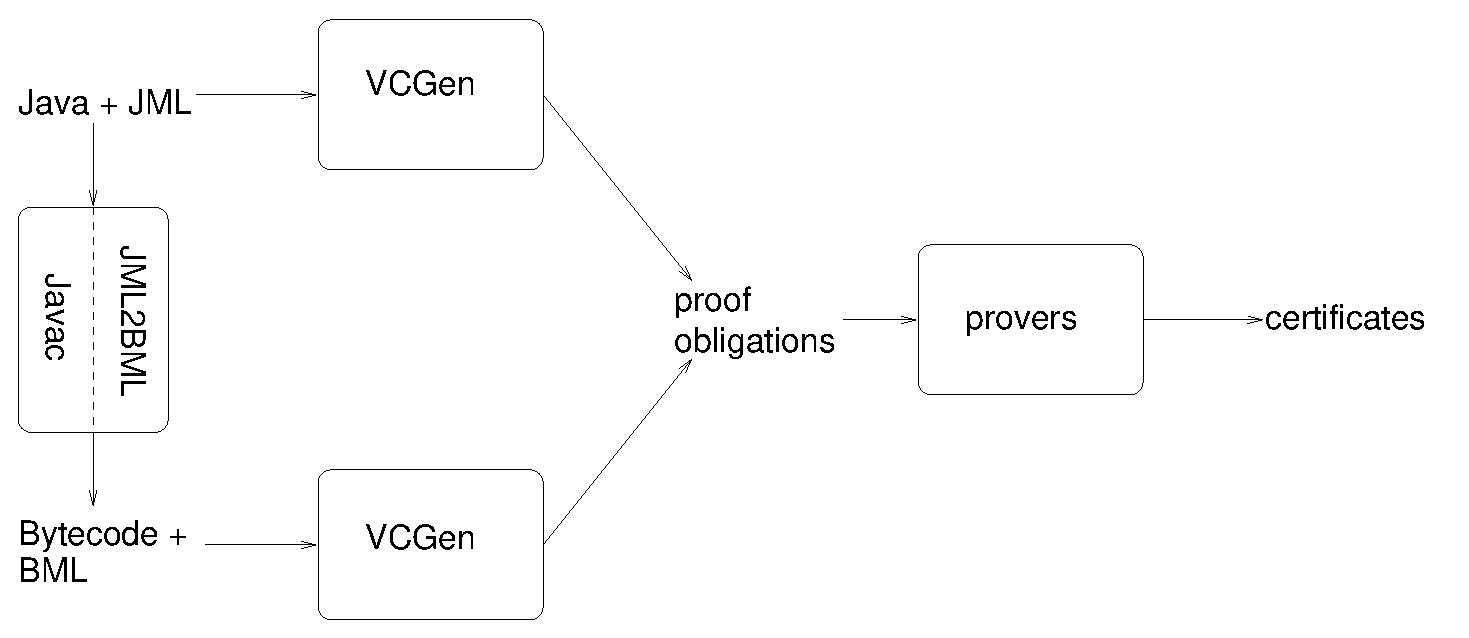
\includegraphics[width=\textwidth]{toolset.eps} 
\caption{Overview of \mobius tool set}\label{FigToolSet}
\end{figure}
As part of the \mobius project, we plan to develop a tool set that
supports both JML and BML. Figure~\ref{FigToolSet} outlines the
general architecture of this tool set. Thus, both Java/JML and
bytecode/BML can be used as input application. For both specification
languages, verification condition generators are used to generate
appropriate proof obligations that can be discharged with a theorem
prover (either automatic or interactive). To support the proof
carrying code platform, the provers will be instrumented to produce
certificates. In addition, source code applications annotated with JML
can be compiled into bytecode annotated with BML.

The development of the JML subcomponent of the tool set will be based
on experiences with ESC/Java~\cite{CokK04} and JACK~\cite{BurdyRL03}.
Several tools and algorithms (notably the compiler and the
verification condition generator) for BML have already been
implemented, see~\cite{BurdyP06}, but more work is needed to cover the
whole language. Moreover, to make the tool set usable in practice, we
will also need a tool to inspect and write directly BML
specifications, and a run-time checker for BML specifications. The
latter can be implemented by a code transformation, inserting explicit
run-time checks in the bytecode, or by extending the virtual machine
to take the user-specific attributes with specifications into account;

Our initial experiments with compilation of specifications has shown
that there exists indeed a correspondence between the proof
obligations generated at source and at bytecode level, modulo
differences in elimination of trivial goals, handling of arithmetic
expressions, and the naming convention of generated
variables. Moreover, when the proofs are done with the Coq prover,
different names are generated for hypotheses at source code and
bytecode level. It is future work to clean up the compilation, so
there is a one-to-one correspondence.




 

\subsection*{Related work}
The interest in specification and verification of bytecode
applications is quite recent, and not too much work has been done in
that direction. Several logics have been developed to reason about
bytecode, \emph{e.g.}~by Bannwart \& M\"uller~\cite{BannwartMueller05}
and within the MRG project~\cite{AspinallEtAl:TPHOLs2004}. However,
in this work, no attention is given to how one can conveniently write
understandable specifications for bytecode.

The development of BML is clearly inspired by the development of the
JML specification language~\cite{JMLReferenceManual05}. Both JML and
BML follow the Design by Contract principle introduced first in
Eiffel~\cite{Meyer97}. The Boogie project~\cite{BarnettCDJL05}
introduces in similarly the Design by Contract principles into the C\#
programming language, both at source code level and for CIL, the .NET
intermediate language.  The possibility to check a property at
run-time, using the \texttt{assert} construct, has been long 
adopted in the C programming language and recently also in Java (Java
1.5, see \cite[\S 14.10]{JLS}). 

Finally, we should mention the Extended Virtual Platform
project\footnote{See
\url{http://www.cs.usm.maine.edu/~mroyer/xvp/}.}. This project aims at
developing a framework that allows to compile JML annotations, to
allow run-time checking~\cite{AlagicXVP05}. However, in contrast to
our work, they do not intend to do static verification of bytecode
programs. Moreover, their platform takes JML-annotated source code
files as starting point, while with BML one is able to annotate
bytecode applications directly\footnote{Some security-critical
applications are written in bytecode directly, to avoid security
problems related with compilation. Thus, for such applications one
needs to be able to specify and verify them directly at this level.}.



\subsection*{Acknowledgements}
We thank Lennart Beringer and Olha Shkaravska for discussions about
the semantics of BML. 




\bibliographystyle{plain}
\bibliography{bytecode,../../THESIS/biblio}

\appendix
% generated and manually adapted from BML-grammar.texinfo

\newdimen{\standardmargin}  \setlength{\standardmargin}{15pt}
\newdimen{\tableindent}     \setlength{\tableindent}{50pt}
\newbox\ItemBox

\setcounter{secnumdepth}{5}       
\setcounter{tocdepth}{5}          

\def\lqHook{\char16 }\def\rqHook{\char17 }\def\lnqHook{\char96 }\def\rnqHook{\char39 }%
%\usepackage{varioref}         




\newcommand{\lbr}{\ifvmode\else\unskip\relax\nobreak\hfil\break\fi}




\newenvironment{display}[1][\standardmargin]%
                       {\begingroup\def~{\mbox{ }}\let\\=\lbr
                        \list{}{\listparindent0pt  \itemindent0pt
                        \rightmargin0pt    \leftmargin#1}%
                \item}
               {\endlist\endgroup}



\renewenvironment{quote}
                 {\list{}{\leftmargin\standardmargin\rightmargin\leftmargin}%
                  \item\relax}
                 {\endlist}



\makeatletter
\newcommand\Nopagebreak{\let\if@nobreak\iftrue \nopagebreak}
\makeatother





\newcommand{\tabletermHook}[1]{#1}

\newcommand{\kbdHook}[1]{\mbox{\ttfamily\slshape #1}}

\newcommand{\keyHook}[1]{{\fboxsep2pt\fbox{\sffamily\footnotesize #1}}}
\newcommand{\sampHook}[1]{\lnqHook\texttt{#1}\rnqHook}
\newcommand{\verbHook}[1]{\mbox{\ttfamily #1}}
\newcommand{\envHook}[1]{\mbox{\ttfamily #1}}
\newcommand{\fileHook}[1]{\lnqHook\texttt{#1}\rnqHook}
\newcommand{\commandHook}[1]{\mbox{\ttfamily #1}}
\newcommand{\optionHook}[1]{\lnqHook\mbox{\ttfamily #1}\rnqHook}
\newcommand{\dfnHook}[1]{\emph{#1}}
\newcommand{\citeHook}[1]{\textit{#1}}
\newcommand{\abbrevwordHook}[1]{#1}
\newcommand{\abbrevdescHook}[1]{ (#1)}
\newcommand{\acronymwordHook}[1]{\mbox{#1}}
\newcommand{\acronymdescHook}[1]{\footnote{#1}}
\newcommand{\urlHook}[1]{#1}
\newcommand{\emailHook}[1]{#1}

\newcommand{\emphHook}[1]{\emph{#1}}
\newcommand{\strongHook}[1]{\textbf{#1}}
\newcommand{\scHook}[1]{\textsc{#1}}
\newcommand{\slantedHook}[1]{\textsl{#1}}
\newcommand{\sansserifHook}[1]{\textsf{#1}}
\newcommand{\iHook}[1]{\textit{#1}}
\newcommand{\bHook}[1]{\textbf{#1}}
\newcommand{\tHook}[1]{\texttt{#1}}
\newcommand{\rHook}[1]{\textrm{#1}}
\newcommand{\dmnHook}[1]{\,\mbox{#1}}
\newcommand{\mathHook}[1]{\ensuremath{#1}}
\newcommand{\footnoteHook}[1]{\footnote{#1}}



\newenvironment{quotationHook}{\begin{quote}}{\end{quote}}
\newenvironment{copyingHook}{\begin{quote}}{\end{quote}}
\newenvironment{verbatimHook}{\begin{display}[0pt]\ttfamily}{\end{display}}
\newenvironment{exampleHook}{\begin{display}\ttfamily}{\end{display}}
\newenvironment{lispHook}{\begin{display}\ttfamily}{\end{display}}
\newenvironment{displayHook}{\begin{display}\relax}{\end{display}}
\newenvironment{formatHook}{\begin{display}[0pt]}{\end{display}}

\newenvironment{smallexampleHook}{\begin{small}\begin{exampleHook}}%
    {\end{exampleHook}\end{small}}
\newenvironment{smalldisplayHook}{\begin{small}\begin{displayHook}}%
    {\end{displayHook}\end{small}}
\newenvironment{smallformatHook}{\begin{small}\begin{formatHook}}%
    {\end{formatHook}\end{small}}
\newenvironment{smalllispHook}{\begin{small}\begin{lispHook}}%
    {\end{lispHook}\end{small}}

\newenvironment{flushleftHook}{\begin{flushleft}}{\end{flushleft}}
\newenvironment{flushrightHook}{\begin{flushright}}{\end{flushright}}
\newenvironment{groupHook}{\begin{samepage}}{\end{samepage}}

\newenvironment{cartoucheHook}{\begin{center}\shadowbox\bgroup
    \hbox to \hsize\bgroup\begin{minipage}{\hsize}}%
    {\end{minipage}\hss\egroup\egroup\end{center}}

\newcommand{\centerHook}[1]{\centerline{#1}}




\newenvironment{definitionitem}[1][\standardmargin]
               {\list{}{\listparindent0pt  \itemindent0pt
                        \rightmargin0pt    \leftmargin#1}%
                \item\removelastskip\relax}
               {\endlist}

\sloppy               
\hbadness20000





%\PassOptionsToPackage{hyphens}{url}
%\newcommand{\xhyphen}{\discretionary{\char127}{}{-}}
%\IfFileExists{pdfcprot.sty}{\usepackage[activate]{pdfcprot}}{}
%\usepackage[%
%  pagebackref=true,pdfstartview=FitH,
%  pdfcreator={texi2latex + LaTeX with hyperref package},
%  pdfpagelayout=OneColumn,
%  bookmarks=true,bookmarksopen=false,  colorlinks,pdfpagelabels=true,
%  draft=false,breaklinks=true,plainpages=false]{hyperref}[2000/05/08]  \hypersetup{%
%    pdftitle={BML grammar},
%    pdfsubject={<setfilename>BML-grammar.texinfo</setfilename>},
%    pdfauthor={}
%  }
%\urlstyle{rm}




%\usepackage{hypbmsec}



%\InputIfFileExists{texi2latex.cfg}%
%  {\message{Loading global configuration file texi2latex.cfg}}{}
%\InputIfFileExists{\jobname-t2l.cfg}%
%  {\message{Loading local configuration file \jobname-t2l.cfg}}{}



%\begin{document}


\gdef\InsertLabelMaybe{\label{predicates-and-specification-expressions}\gdef\InsertLabelMaybe{}}
\section{Grammar for BML predicates and specification expressions}\label{AppBML}\InsertLabelMaybe

\textbf{NOTE: We intend to set up a webpage with the complete BML grammar 
before publication. This grammar is included for the reviewer's
convenience, but will not be included in the final version of the
paper.}

As in the JML Reference Manual~\cite{JMLReferenceManual05}, we use an
extended Backus-Nauer Form (BNF) grammar to describe the syntax of
JML. The extensions are as follows~\cite{Ledgard80}.

\begin{itemize}
\item Nonterminal symbols are written as follows: \varHook{nonterminal}.

\item Terminal symbols are written as follows: \codeHook{terminal}.

\item Square brackets ([ and ]) surround optional text. Notice that
\codeHook{[} and \codeHook{]} are terminal symbols.  

\item The notation \dots\ means that the preceding nonterminal or group of optional text can be repeated zero or more times.  
\end{itemize}

\begin{displayHook}\\\relax {\varHook{predicate}}~::=~{\varHook{spec-{}expression}}\\\relax {\varHook{spec-{}expression-{}list}}~::=~{\varHook{spec-{}expression}}\\\relax ~~~~~~~~~~~~~~~~~~~~~~~~~[~{\codeHook{,}}~{\varHook{spec-{}expression}}~]~\dots \@{}\\\relax {\varHook{spec-{}expression}}~::=~{\varHook{expression}}\\\relax {\varHook{expression-{}list}}~::=~{\varHook{expression}}~[~{\codeHook{,}}~{\varHook{expression}}~]~\dots \@{}\\\relax {\varHook{expression}}~::=~{\varHook{conditional-{}expr}}~\\\relax {\varHook{conditional-{}expr}}~::=~{\varHook{equivalence-{}expr}}\\\relax ~~~~~~~~~~~~~~~~~~~[~{\codeHook{?{}}}~{\varHook{conditional-{}expr}}~{\codeHook{:}}~{\varHook{conditional-{}expr}}~]\\\relax {\varHook{equivalence-{}expr}}~::=~{\varHook{implies-{}expr}}\\\relax ~~~~~~~~~~~~~~~~~~~~~[~{\varHook{equivalence-{}op}}~{\varHook{implies-{}expr}}~]~\dots \@{}\\\relax {\varHook{equivalence-{}op}}~::=~{\codeHook{<{}==>{}}}~{\mbox{\char124{}}}~{\codeHook{<{}=!{}=>{}}}\\\relax {\varHook{implies-{}expr}}~::=~{\varHook{logical-{}or-{}expr}}\\\relax ~~~~~~~~~~~~~[~{\codeHook{==>{}}}~{\varHook{implies-{}non-{}backward-{}expr}}~]\\\relax ~~~~~~~~{\mbox{\char124{}}}~{\varHook{logical-{}or-{}expr}}~{\codeHook{<{}==}}~{\varHook{logical-{}or-{}expr}}\\\relax ~~~~~~~~~~~~~[~{\codeHook{<{}==}}~{\varHook{logical-{}or-{}expr}}~]~\dots \@{}\\\relax {\varHook{implies-{}non-{}backward-{}expr}}~::=~{\varHook{logical-{}or-{}expr}}\\\relax ~~~~~~~~~~~~~[~{\codeHook{==>{}}}~{\varHook{implies-{}non-{}backward-{}expr}}~]\\\relax {\varHook{logical-{}or-{}expr}}~::=~{\varHook{logical-{}and-{}expr}}~[~`{}{\codeHook{{\mbox{\char124{}}}{\mbox{\char124{}}}}}'{}~{\varHook{logical-{}and-{}expr}}~]~\dots \@{}\\\relax {\varHook{logical-{}and-{}expr}}~::=~{\varHook{inclusive-{}or-{}expr}}~[~{\codeHook{\&\&}}~{\varHook{inclusive-{}or-{}expr}}~]~\dots \@{}\\\relax {\varHook{inclusive-{}or-{}expr}}~::=~{\varHook{exclusive-{}or-{}expr}}~[~`{}{\codeHook{{\mbox{\char124{}}}}}'{}~{\varHook{exclusive-{}or-{}expr}}~]~\dots \@{}\\\relax {\varHook{exclusive-{}or-{}expr}}~::=~{\varHook{and-{}expr}}~[~{\codeHook{{\mbox{\char94{}}}}}~{\varHook{and-{}expr}}~]~\dots \@{}\\\relax {\varHook{and-{}expr}}~::=~{\varHook{equality-{}expr}}~[~{\codeHook{\&}}~{\varHook{equality-{}expr}}~]~\dots \@{}\\\relax {\varHook{equality-{}expr}}~::=~{\varHook{relational-{}expr}}~[~{\codeHook{==}}~{\varHook{relational-{}expr}}]~\dots \@{}\\\relax ~~~~~~~~{\mbox{\char124{}}}~{\varHook{relational-{}expr}}~[~{\codeHook{!{}=}}~{\varHook{relational-{}expr}}]~\dots \@{}\\\relax {\varHook{relational-{}expr}}~::=~{\varHook{shift-{}expr}}~{\codeHook{<{}}}~{\varHook{shift-{}expr}}\\\relax ~~~~~~~~{\mbox{\char124{}}}~{\varHook{shift-{}expr}}~{\codeHook{>{}}}~{\varHook{shift-{}expr}}\\\relax ~~~~~~~~{\mbox{\char124{}}}~{\varHook{shift-{}expr}}~{\codeHook{<{}=}}~{\varHook{shift-{}expr}}\\\relax ~~~~~~~~{\mbox{\char124{}}}~{\varHook{shift-{}expr}}~{\codeHook{>{}=}}~{\varHook{shift-{}expr}}\\\relax ~~~~~~~~{\mbox{\char124{}}}~{\varHook{shift-{}expr}}~{\codeHook{<{}:}}~{\varHook{shift-{}expr}}\\\relax ~~~~~~~~{\mbox{\char124{}}}~{\varHook{shift-{}expr}}~[~{\codeHook{instanceof}}~{\varHook{type-{}spec}}~]\\\relax {\varHook{shift-{}expr}}~::=~{\varHook{additive-{}expr}}~[~{\varHook{shift-{}op}}~{\varHook{additive-{}expr}}~]~\dots \@{}\\\relax {\varHook{shift-{}op}}~::=~{\codeHook{<{}<{}}}~{\mbox{\char124{}}}~{\codeHook{>{}>{}}}~{\mbox{\char124{}}}~{\codeHook{>{}>{}>{}}}\\\relax {\varHook{additive-{}expr}}~::=~{\varHook{mult-{}expr}}~[~{\varHook{additive-{}op}}~{\varHook{mult-{}expr}}~]~\dots \@{}\\\relax {\varHook{additive-{}op}}~::=~{\codeHook{+}}~{\mbox{\char124{}}}~{\codeHook{-{}}}\\\relax {\varHook{mult-{}expr}}~::=~{\varHook{unary-{}expr}}~[~{\varHook{mult-{}op}}~{\varHook{unary-{}expr}}~]~\dots \@{}\\\relax {\varHook{mult-{}op}}~::=~{\codeHook{*}}~{\mbox{\char124{}}}~{\codeHook{/}}~{\mbox{\char124{}}}~{\codeHook{\%}}\\\relax {\varHook{unary-{}expr}}~::=~{\codeHook{(}}~{\varHook{type-{}spec}}~{\codeHook{)}}~{\varHook{unary-{}expr}}\\\relax ~~~~~~~~{\mbox{\char124{}}}~{\codeHook{+}}~{\varHook{unary-{}expr}}\\\relax ~~~~~~~~{\mbox{\char124{}}}~{\codeHook{-{}}}~{\varHook{unary-{}expr}}\\\relax ~~~~~~~~{\mbox{\char124{}}}~{\varHook{unary-{}expr-{}not-{}plus-{}minus}}\\\relax {\varHook{unary-{}expr-{}not-{}plus-{}minus}}~::=~{\codeHook{{\mbox{\char126{}}}}}~{\varHook{unary-{}expr}}\\\relax ~~~~~~~~{\mbox{\char124{}}}~{\codeHook{!{}}}~{\varHook{unary-{}expr}}\\\relax ~~~~~~~~{\mbox{\char124{}}}~{\codeHook{(}}~{\varHook{built-{}in-{}type}}~{\codeHook{)}}~{\varHook{unary-{}expr}}\\\relax ~~~~~~~~{\mbox{\char124{}}}~{\codeHook{(}}~{\varHook{reference-{}type}}~{\codeHook{)}}~{\varHook{unary-{}expr-{}not-{}plus-{}minus}}\\\relax ~~~~~~~~{\mbox{\char124{}}}~{\varHook{primary-{}expr}}~[~{\varHook{primary-{}suffix}}~]~\dots \@{}\\\relax {\varHook{primary-{}suffix}}~::=~{\codeHook{(}}~[~{\varHook{expression-{}list}}~]~{\codeHook{)}}\\\relax ~~~~~~~~{\mbox{\char124{}}}~`{}{\codeHook{[}}'{}~{\varHook{expression}}~`{}{\codeHook{]}}'{}\\\relax {\varHook{primary-{}expr}}~::=~~{\codeHook{{\mbox{\char92{}}}{\mbox{\char35{}}}}}{\varHook{natural}}~{\mbox{\char124{}}}~{\codeHook{lv[}}~{\varHook{natural}}~{\codeHook{]}}\\\relax ~~~~~~~~{\mbox{\char124{}}}~{\varHook{constant}}~{\mbox{\char124{}}}~{\codeHook{super}}~{\mbox{\char124{}}}~{\codeHook{true}}\\\relax ~~~~~~~~{\mbox{\char124{}}}~{\codeHook{false}}~{\mbox{\char124{}}}~{\codeHook{this}}~{\mbox{\char124{}}}~{\codeHook{null}}\\\relax ~~~~~~~~{\mbox{\char124{}}}~{\codeHook{(}}~{\varHook{expression}}~{\codeHook{)}}\\\relax ~~~~~~~~{\mbox{\char124{}}}~{\varHook{bml-{}primary}}\\\relax ~~~~~~~~{\mbox{\char124{}}}~{\varHook{jml-{}primary}}\\\relax {\varHook{built-{}in-{}type}}~::=~{\codeHook{void}}~{\mbox{\char124{}}}~{\codeHook{boolean}}~{\mbox{\char124{}}}~{\codeHook{byte}}\\\relax ~~~~~~~~{\mbox{\char124{}}}~{\codeHook{char}}~{\mbox{\char124{}}}~{\codeHook{short}}~{\mbox{\char124{}}}~{\codeHook{int}}\\\relax ~~~~~~~~{\mbox{\char124{}}}~{\codeHook{long}}~{\mbox{\char124{}}}~{\codeHook{float}}~{\mbox{\char124{}}}~{\codeHook{double}}\\\relax {\varHook{constant}}~::=~{\varHook{java-{}literal}}\\\relax {\varHook{bml-{}primary}}~::=~{\varHook{array-{}length-{}expression}}~{\mbox{\char124{}}}\\\relax ~~~~~~~~~~~{\mbox{\char124{}}}~{\varHook{opstack-{}counter-{}expression}}\\\relax ~~~~~~~~~~~{\mbox{\char124{}}}~{\varHook{stack-{}expresion}}\\\relax {\varHook{array-{}length-{}expression}}~::=~{\codeHook{length(}}~{\varHook{expression}}~{\codeHook{)}}\\\relax {\varHook{opstack-{}counter-{}expression}}~::=~{\codeHook{cntr}}\\\relax {\varHook{stack-{}expression}}~::=~{\codeHook{st(}}~{\varHook{additive-{}expr}}~{\codeHook{)}}\\\relax {\varHook{jml-{}primary}}~::=~{\varHook{result-{}expression}}\\\relax ~~~~~~~~{\mbox{\char124{}}}~{\varHook{old-{}expression}}\\\relax ~~~~~~~~{\mbox{\char124{}}}~{\varHook{fresh-{}expression}}\\\relax ~~~~~~~~{\mbox{\char124{}}}~{\varHook{nonnullelements-{}expression}}\\\relax ~~~~~~~~{\mbox{\char124{}}}~{\varHook{typeof-{}expression}}\\\relax ~~~~~~~~{\mbox{\char124{}}}~{\varHook{elemtype-{}expression}}\\\relax ~~~~~~~~{\mbox{\char124{}}}~{\varHook{type-{}expression}}\\\relax ~~~~~~~~{\mbox{\char124{}}}~{\varHook{spec-{}quantified-{}expr}}\\\relax {\varHook{result-{}expression}}~::=~{\codeHook{{\mbox{\char92{}}}result}}\\\relax {\varHook{old-{}expression}}~::=~{\codeHook{{\mbox{\char92{}}}old}}~{\codeHook{(}}~{\varHook{spec-{}expression}}~{\codeHook{)}}\\\relax ~~~~~~~~{\mbox{\char124{}}}~{\codeHook{{\mbox{\char92{}}}pre}}~{\codeHook{(}}~{\varHook{spec-{}expression}}~{\codeHook{)}}\\\relax {\varHook{fresh-{}expression}}~::=~{\codeHook{{\mbox{\char92{}}}fresh}}~{\codeHook{(}}~{\varHook{spec-{}expression-{}list}}~{\codeHook{)}}\\\relax {\varHook{nonnullelements-{}expression}}~::=~{\codeHook{{\mbox{\char92{}}}nonnullelements}}~{\codeHook{(}}~{\varHook{spec-{}expression}}~{\codeHook{)}}\\\relax {\varHook{typeof-{}expression}}~::=~{\codeHook{{\mbox{\char92{}}}typeof}}~{\codeHook{(}}~{\varHook{spec-{}expression}}~{\codeHook{)}}\\\relax {\varHook{elemtype-{}expression}}~::=~{\codeHook{{\mbox{\char92{}}}elemtype}}~{\codeHook{(}}~{\varHook{spec-{}expression}}~{\codeHook{)}}\\\relax {\varHook{type-{}expression}}~::=~{\codeHook{{\mbox{\char92{}}}type}}~{\codeHook{(}}~{\varHook{type}}~{\codeHook{)}}\\\relax {\varHook{spec-{}quantified-{}expr}}~::=~{\codeHook{(}}~{\varHook{quantifier}}~{\varHook{quantified-{}var-{}decls}}~{\codeHook{;}}\\\relax ~~~~~~~~~~~~~~~~~~~~~~~~~~~[~[~{\varHook{predicate}}~]~{\codeHook{;}}~]\\\relax ~~~~~~~~~~~~~~~~~~~~~~~~~~~{\varHook{spec-{}expression}}~{\codeHook{)}}\\\relax {\varHook{quantifier}}~::=~{\codeHook{{\mbox{\char92{}}}forall}}~{\mbox{\char124{}}}~{\codeHook{{\mbox{\char92{}}}exists}}\\\relax {\varHook{quantified-{}var-{}decls}}~::=~[~{\varHook{bound-{}var-{}modifiers}}~]~{\varHook{type-{}spec}}~{\varHook{quantified-{}var-{}declarator}}\\\relax ~~~~~~~~~~~~~~~~~~~~~~~~~[~{\codeHook{,}}~{\varHook{quantified-{}var-{}declarator}}~]~\dots \@{}\\\relax {\varHook{quantified-{}var-{}declarator}}~::=~{\varHook{ident}}~[~{\varHook{dims}}~]\\\relax {\varHook{bound-{}var-{}modifiers}}~::=~{\codeHook{non{\mbox{\char95{}}}null}}~{\mbox{\char124{}}}~{\codeHook{nullable}}\\\relax {\varHook{store-{}ref-{}list}}~::=~{\varHook{store-{}ref}}~[~{\codeHook{,}}~{\varHook{store-{}ref}}~]~\dots \@{}\\\relax {\varHook{store-{}ref}}~::=~{\varHook{store-{}ref-{}expression}}\\\relax ~~~~~~~~{\mbox{\char124{}}}~{\varHook{store-{}ref-{}keyword}}\\\relax {\varHook{store-{}ref-{}expression}}~::=~{\varHook{store-{}ref-{}name}}~[~{\varHook{store-{}ref-{}name-{}suffix}}~]~\dots \@{}\\\relax {\varHook{store-{}ref-{}name}}~::=~{\codeHook{{\mbox{\char92{}}}{\mbox{\char35{}}}}}~{\varHook{natural}}~{\mbox{\char124{}}}~{\codeHook{super}}~{\mbox{\char124{}}}~{\codeHook{this}}\\\relax {\varHook{store-{}ref-{}name-{}suffix}}~::=~{\codeHook{(}}~{\varHook{store-{}ref-{}expression}}~{\codeHook{)}}\\\relax ~~~~~~~~{\mbox{\char124{}}}~`{}{\codeHook{[}}'{}~{\varHook{spec-{}array-{}ref-{}expr}}~`{}{\codeHook{]}}'{}\\\relax {\varHook{spec-{}array-{}ref-{}expr}}~::=~{\varHook{spec-{}expression}}\\\relax ~~~~~~~~{\mbox{\char124{}}}~{\varHook{spec-{}expression}}~{\codeHook{..}}~{\varHook{spec-{}expression}}\\\relax ~~~~~~~~{\mbox{\char124{}}}~{\codeHook{*}}\\\relax {\varHook{store-{}ref-{}keyword}}~::=~{\codeHook{{\mbox{\char92{}}}nothing}}~{\mbox{\char124{}}}~{\codeHook{{\mbox{\char92{}}}everything}}~{\mbox{\char124{}}}~{\codeHook{{\mbox{\char92{}}}not{\mbox{\char95{}}}specified}}\end{displayHook}


\end{document}
